%!TEX root = Constructive Alignment for Introductory Programming.tex

\chapter{A Model for Constructive Alignment of Introductory Programming} % (fold)
\label{cha:approach}

\graphicspath{{Figures/CAApproach/}}

\cref{cha:guiding_principles} outlined twelve principles, nine for guiding \emph{how} to create a student-centred learning environment, and three for guiding decisions on \emph{what} should be taught in introductory programming. This chapter proposes a model for applying constructive alignment for teaching introductory programming that is in agreement with the twelve principles.

\sref{sec:overall_strategy} describes an application of the principles in defining the overall strategy for teaching introductory programming, outlining the assessment approach used and the approach taken to deliver this material in a student centred manner. This section argues for the user of portfolio assessment, and provides some guidelines for designing and delivering lecture and tutorial classes. Following this, the general model for constructive alignment is presented in \sref{sec:model}, which describes the overall model, the processes within it, and means for addressing plagiarism. The chapter concludes with a brief summary in \sref{sec:ca_summary}.

\section{Overall Strategy} % (fold)
\label{sec:overall_strategy}

One of the overarching principles from \cref{cha:guiding_principles} is the requirement to be agile and willing to change (\pref{itm:agile}). In discussing this principle, \sref{ssub:be_agile_and_willing_to_change} outlined that teaching and learning resources need to be guided by an overall strategy. The overall strategy informs, and is shaped by, the assessment approach, approach to material delivery, and the approach to the selection of unit content. This section describes the application of the principles from \cref{cha:guiding_principles} to the selection of an assessment approach and approach to material delivery. The discussion of approach to selecting content, and specific intended learning outcomes that follow, are presented in \cref{cha:example_impl}.

\subsection{Assessment Approach} % (fold)
\label{sub:assessment_approach}

Assessment plays an important role in defining what students learn. \citet{Rowntree:1977} indicated the central role of assessment procedures in understanding any education system. This is supported by \citet{Ramsden:2003}, who stated that ``from our students' point of view, assessment always defines the actual curriculum'', and further supported by \citet{Biggs:2007} who indicated that ``students learn what they \emph{think} they will be tested on.'' In presenting their conditions for effective assessment, \citet{Gibbs:2004} discussed the dominant influence of assessment in defining what students focus on, indicating that students are able to distinguish between what assessment requires them to pay attention to, and what is likely to result in effective learning. So the selection of an assessment approach will have a significant impact on the overall strategy for both students and staff. 

Consider a traditional introductory programming, taught using a number of assignments and a final examination. This approach, while commonly used, is not in keeping with several of our guiding principles, as outlined in the following list. 

\begin{enumerate}[noitemsep,nolistsep]
	\item This approach to assessment is teacher-centred, and does not easily incorporate aspects from constructive learning theory, as discussed in \cref{cha:background}.  As a result, some adjustments are required in order to address \pref{itm:construct}.
	\item The teacher-centred nature of the assessment also excludes students from the alignment process, \pref{itm:align}, with staff performing the alignment of assessment tasks with intended learning outcomes resulting in additional opportunities for misalignment, as discussed in \cref{cha:background}. 
	\item Similarly, the use of summative assessment during the semester goes against \pref{itm:formative} with its goal of assessing outcomes, and using frequent formative feedback to aid student learning.
	\item The use of assignments marks to motivate students is also contrary to \pref{itm:theory_y}, with marks being used for motivation in either a hard or soft form of Theory X strategy.
	\item Marked assignments also indicate a finality, with marks being lost or gained when the assignment is assessed. These results are typically final, and therefore provide no incentive for student to reflect on their approach to learning, and to ensure they have more fully understood concepts before proceeding. Alternate assessment strategies, with a greater emphasis on formative feedback, could better encapsulate the ideals of reflective practice, and thereby better meet \pref{itm:reflect}.
\end{enumerate}

As a result, the principles from \cref{cha:guiding_principles} requires us to consider other forms of assessment.
  
%
% this is commonly done e.g. in German universities - and sometimes exams
%  are delayed to a later YEAR (let alone end of unit)...
%

One strategy to address this would be to abandon coursework assignments, delaying final summative assessment to an examination worth 100\% of the student's grade. While this would address \pref{itm:formative}, such a heavy weight examination is very much a hard Theory X approach, and fails to recognise the value of coursework assignments, which have been strongly argued for as in \citet{Gibbs:2004} which provided several strong arguments for coursework assignments, including the following:
\begin{itemize}[noitemsep,nolistsep]
	\item Units that include coursework assignments, in addition to an exam, resulted in higher average marks than compared with units that included no coursework assignments \cite{Chansarkar:1987}.
	\item Students prefer coursework assignments over examinations. A position that is also supported by \citet{Kniveton:1996} who stated that students prefer coursework assignments to exams as assignments assessed a better range of their abilities and enabled them to organise their time to a greater extent.
	\item Students attain better results from coursework than examinations. \citet{Gibbs:1997} indicated a strong positive correlation between the proportion of coursework assignments and average marks. Though, \citet{James:2004} indicated that individual students do not consistently perform better, or worse, on any one form of assessment.
	\item Coursework assignments are at least as valid a form of assessment as examinations:
	\begin{itemize}[noitemsep,nolistsep]
	% 
	% Do you have reference to support this statement: 
	% AC: yes :)
		\item Exams are a poor predictor of future performance \cite{Baird:1985,Gibbs:2004}.
		\item Coursework assignments are a better predictor of long term learning than exam results \cite{Conway:1992}. This supports the idea that students adopt surface approaches to preparing for exams \citet{Marton:1976a, Tang:1999}. 
		%
		% Ditto  - reference(s) to support this needed here ->
		%
		\item The quality of learning is deeper in assignment-based units, when compared to exam-based units \cite{Tynjala:1998,Gibbs:2004}.
	\end{itemize}
\end{itemize}

The challenge, therefore, is to define an assessment approach that enables students to construct their knowledge, uses coursework assignments in a formative manner, and enables 100\% of each student's grade to be determined after the end of the teaching period, with a strong alignment to unit intended learning outcomes.

\clearpage
\subsubsection{Portfolio Assessment} % (fold)
\label{sub:portfolio_assessment}

In proposing Constructive Alignment, \citet{Biggs:1996c} advocated strongly for the use of an assessment portfolio, and indicated that the principles of constructive alignment had evolved with the decision to use portfolio assessment. This work was extended in his later work, presented in \cite{Biggs:1997}, which outlined suggestions for implementing portfolio assessment and a generalised model for instruction design. Further advice and details of the generalised model were presented in \citet{Biggs:2007} book on quality learning at university.

Assessment involves three components, all of which are typically under the control of the teacher \cite{Biggs:1997}. These include \emph{setting criteria}, \emph{selecting evidence} and \emph{making a judgement}. With the assessment portfolio the students take control of \emph{at least} the selection of evidence, as illustrated in \fref{fig:select_evidence}. The portfolio is then a collection of work that the student puts forward for assessment against the unit's intended learning outcomes, which helps avoid the teacher-selected \emph{sampling} effect of exams.

\begin{figure}[htbp]
	\centering
	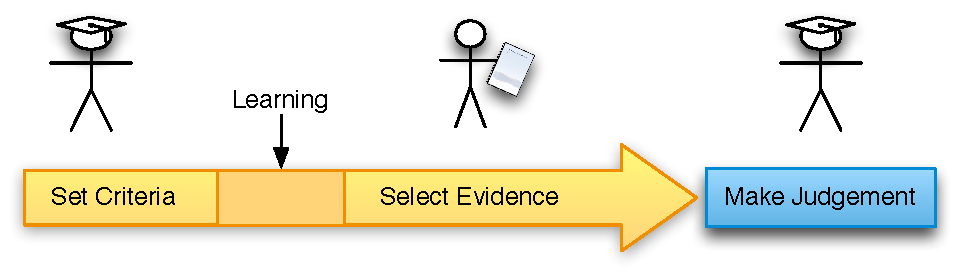
\includegraphics[width=0.8\textwidth]{SelectEvidence}
	\caption{With portfolio assessment the student is responsible for, at least, the selection of evidence in the assessment process.}
	\label{fig:select_evidence}
\end{figure}

%
% Could note that this approach has been used in Architecture and DEsign areas for many years??
% 

\citet{Smith:2001,Smith:2003} identified four different kinds of portfolios evident in the research literature: \emph{dossier}, \emph{reflective}, \emph{training} and \emph{personal development}. These reflect the combination of two identified factors: (a) the purpose of the portfolio as either for selection/promotion or learning, and (b) whether the portfolio is self-directed or mandated. The details of these are described in the following list, and shown in \fref{fig:portfolio_types}.

\begin{description}[noitemsep,nolistsep]
	\item[Dossier] [selection/promotion, mandated] is a portfolio for the purpose of selection or promotion that contains a mandated collection of work to demonstrate achievement. 
	\item[Reflective] portfolios [selection/promotion, self-directed] contain a self selected collection of work that demonstrates growth or accomplishment for the purpose of admission or promotion. The portfolio is accompanied by a self-appraisal, with the justification for the selection of pieces being as important as the evidence itself.
	\item[Training] portfolios [learning, mandated] are a mandated collection of work performed in a learning context. The portfolio has a fixed format, and contains representative work from the student demonstrating acquired skills, knowledge and competencies.
	\item[Personal development] portfolios [learning, self-directed] are a self-selected collection of work, and reflective account of personal growth over an extended period.
\end{description}

\begin{figure}[htbp]
	\centering
	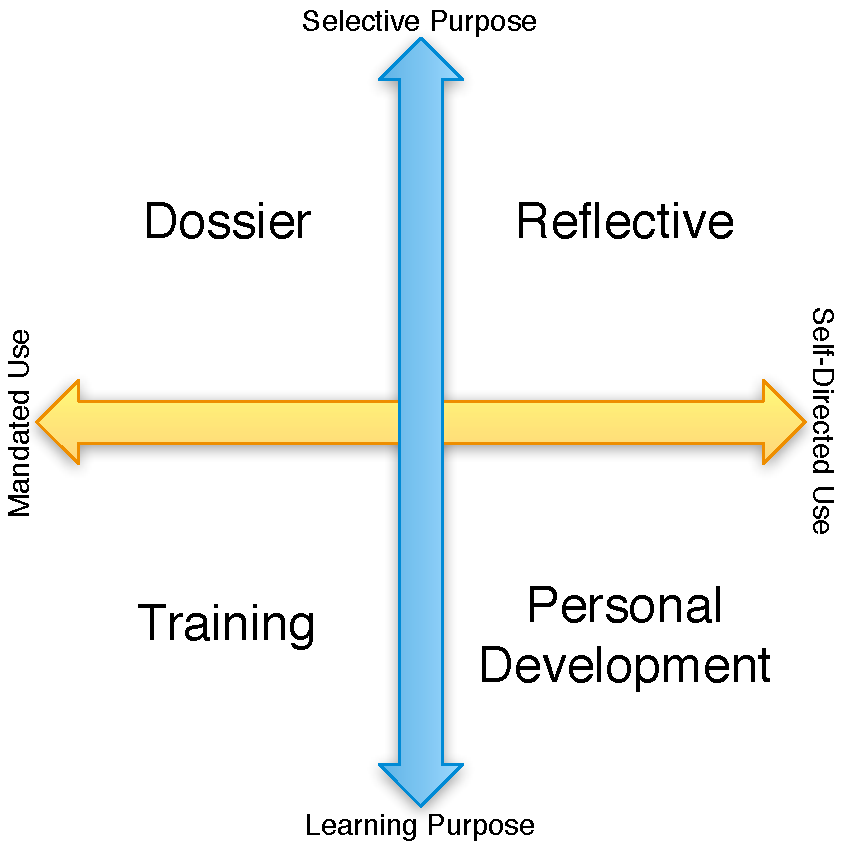
\includegraphics[width=0.50\textwidth]{PortfolioTypes}
	\caption{The four kinds of portfolio based upon purpose and use from \citet{Smith:2001}.}
	\label{fig:portfolio_types}
\end{figure}

Biggs' use of an \emph{assessment portfolio} clearly fits with the \emph{Training} portfolio classification, being a mandated part of the unit assessment for the purpose of evaluating learning outcomes. In the study of a small group of professionals, \citet{Smith:2001} found the training portfolio to be highly rated. Their findings indicated that students found the training portfolio confusing initially, but that once they had understood its function and rational they liked the approach, were easily able to construct their portfolio, and felt it was a fair way to assess their learning.

\citet{Tang:1999} provides further evidence of the value of portfolio assessment. In evaluating how students approach study, they found that students tended to have a narrow, surface approach to studying for tests. These same students were found to adopt wider, more cognitively challenging, approaches when preparing for a portfolio assessment. 

Portfolios have been used to before to assess introductory programming. \cite{Plimmer:2000} reported the successful use of portfolio assessment in an introductory programming unit in which the portfolio contributed between 25\% and 60\% of the students' final grades. Programming portfolios were also discussed by \cite{Jones:2010}, where students submitted a number of portfolio assignments during the semester. These two approaches represent interesting applications of portfolio assessment, but do not use the portfolio as a means of performing a holistic assessment of the students ability to meet the intended learning outcomes, as is proposed in this work.


%
%  Reference if these are quotes?
%  AC: our statement

We argue that when used as a holistic assessment of student performances, portfolio assessment enables a shift from a Theory X ``sage on the stage'' view, to a Theory Y ``guide by the side'' view of education. The traditional approach of setting assignments and exams, in which educators test student ability, becomes inverted with portfolio assessment. Details of the assessment are no longer hidden, as is the case with exams, but is shared with students as the goal they need to achieve. Using portfolio assessment, the emphasis is on the students, and it is their responsibility to demonstrate how they have met a unit's intended learning outcomes. This frees educators to help students and to guide them in the preparation of their evidence. As illustrated in \fref{fig:sage_guide}, we are now working side by side with the students, helping them to achieve the unit's intended learning outcomes. 

\begin{figure}[hb]
	\centering
	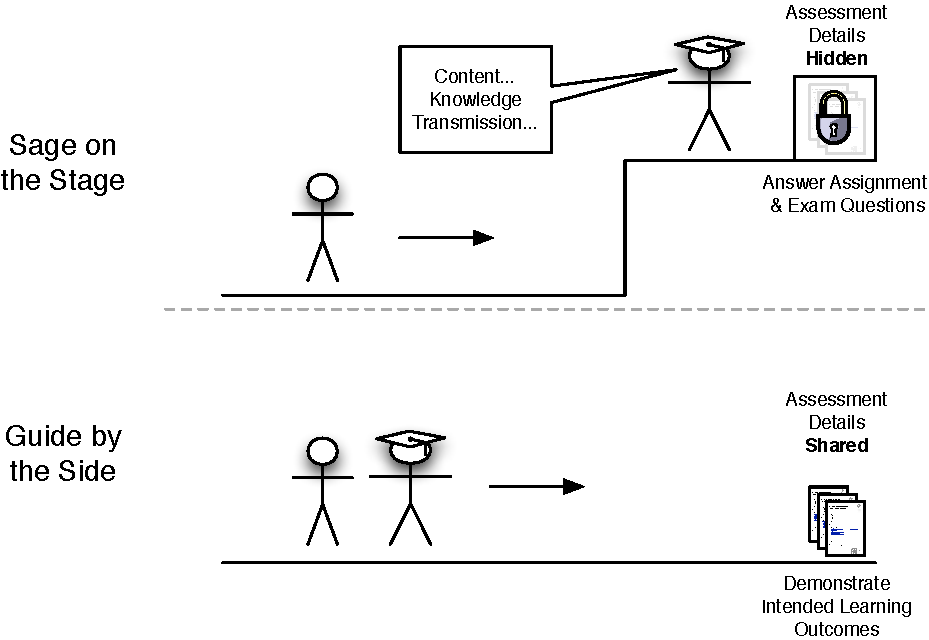
\includegraphics[width=0.90\textwidth]{SageGuide}
	\caption{Portfolio assessment helps enable the view of teaching staff as acting as a ``guide by the side'', rather than a ``sage of the stage''}
	\label{fig:sage_guide}
\end{figure}

%
% This is GOOD!!
%
\clearpage
Portfolio assessment aligns well with all nine ``\emph{how}'' principles listed in \cref{cha:guiding_principles}. 
\begin{itemize}[noitemsep,nolistsep]
	\item The portfolio consists of a collection of work the student feels demonstrates the depth of their knowledge. (\Pref{itm:construct})
	\item Assessment criteria for the portfolio can be aligned with the unit's intended learning outcomes. (\Pref{itm:align})
	\item The portfolio can be used as the sole form of summative assessment, with students being able to take advantage of formative feedback throughout the teaching period. (\Pref{itm:formative})
	\item A clear focus, and use of verbs from the relevant levels of the SOLO taxonomy, will ensure the portfolio requires students to engage appropriate cognitive levels, requiring them to explain, justify and reflect in cases where a depth of understanding is required. (\Pref{itm:focus})
	\item By communicating high expectations, students will strive to create high quality evidence for their portfolios. (\Pref{itm:expectations})
	\item Students are able to develop evidence for their portfolio from day one; everything they do could be of value. This will require active support from teaching staff. (\Pref{itm:support})
	\item Without marks for motivation, an entirely portfolio assessed unit empowers students in the learning process, and they must be trusted that they are able to effectively manage their own learning. (\Pref{itm:theory_y})
	\item Portfolio assessment, with frequent formative feedback, is very much akin to agile software development processes. In addition, student portfolios provide a wealth of evidence for educators to guide change. (\Pref{itm:agile})
	\item Incorporating a reflective component in the portfolio encourages students to engage in reflective practice. (\Pref{itm:reflect})
\end{itemize}

Given its role in the formation of constructive alignment, and its clear alignment with the principles from \cref{cha:guiding_principles}, the approach to constructive alignment for introductory programming presented in this chapter uses portfolio assessment.

%
% Question - maybe need to answer here, later in this chapter or in discussion chapter:
%
% MUST such an approach use portfolio???  i.e. could adopting the principles
% be applied to project or mixed-mode assessment???
% AC: discussion - we tried several variations ... and we feel it does need to be like this
% 

% subsection portfolio_assessment (end)
% subsection assessment_approach (end)

\clearpage
\subsection{Delivery Approach} % (fold)
\label{sub:delivery_approach}

The second aspect of the overall strategy is to define an approach for selecting unit content, with \pref{itm:paradigm} indicating that the overall strategy needs to be defined around a programming paradigm. Rather than focusing on the specific question of which programming paradigm, objects-first or objects-later, was chosen in this work, this section will demonstrate how the principles from \cref{cha:guiding_principles} guide the design and delivery of teaching and learning activities. These guidelines apply equally to both approaches, and a range of other teaching and learning contexts. The specifics of the chosen paradigm for the example implementations is presented in \sref{sec:paradigm_choice} of \cref{cha:example_impl}.

A range of teaching and learning activities are appropriate for helping students develop an understanding of introductory programming. In the following sections we illustrate how the principles from \cref{cha:guiding_principles} can be used to focus lecture away from knowledge transmission, and provide structured learning in laboratory sessions.

\subsubsection{Focused Lecture Slides} % (fold)
\label{ssub:lecture_slides}

\pref{itm:concepts} and \pref{itm:authentic} proposed a concept-based approach to teaching introductory programming content. These principles, along with \pref{itm:focus}, guided the choice to use the ``Beyond Bullet Points'' style of presentation for lectures \cite{Atkinson:2007}. This approach draws upon the work of Richard Mayer (see \citet{Mayer:2005}), and structures presentations using a storyboard that guides the audience toward a stated ``solution''. Using this structure helps to enable a shift in focus, from presentations as providing information to presentations as providing cognitive guidance, where the aim of the presentation is to guide the audience to build appropriate knowledge. An example of the storyboard template, outlining a presentation on arrays, is shown in \fref{fig:bbp}. This story guided the audience to the solution ``Use arrays to store multiple values in a single variable.''

\begin{figure}[htbp]
	\centering
	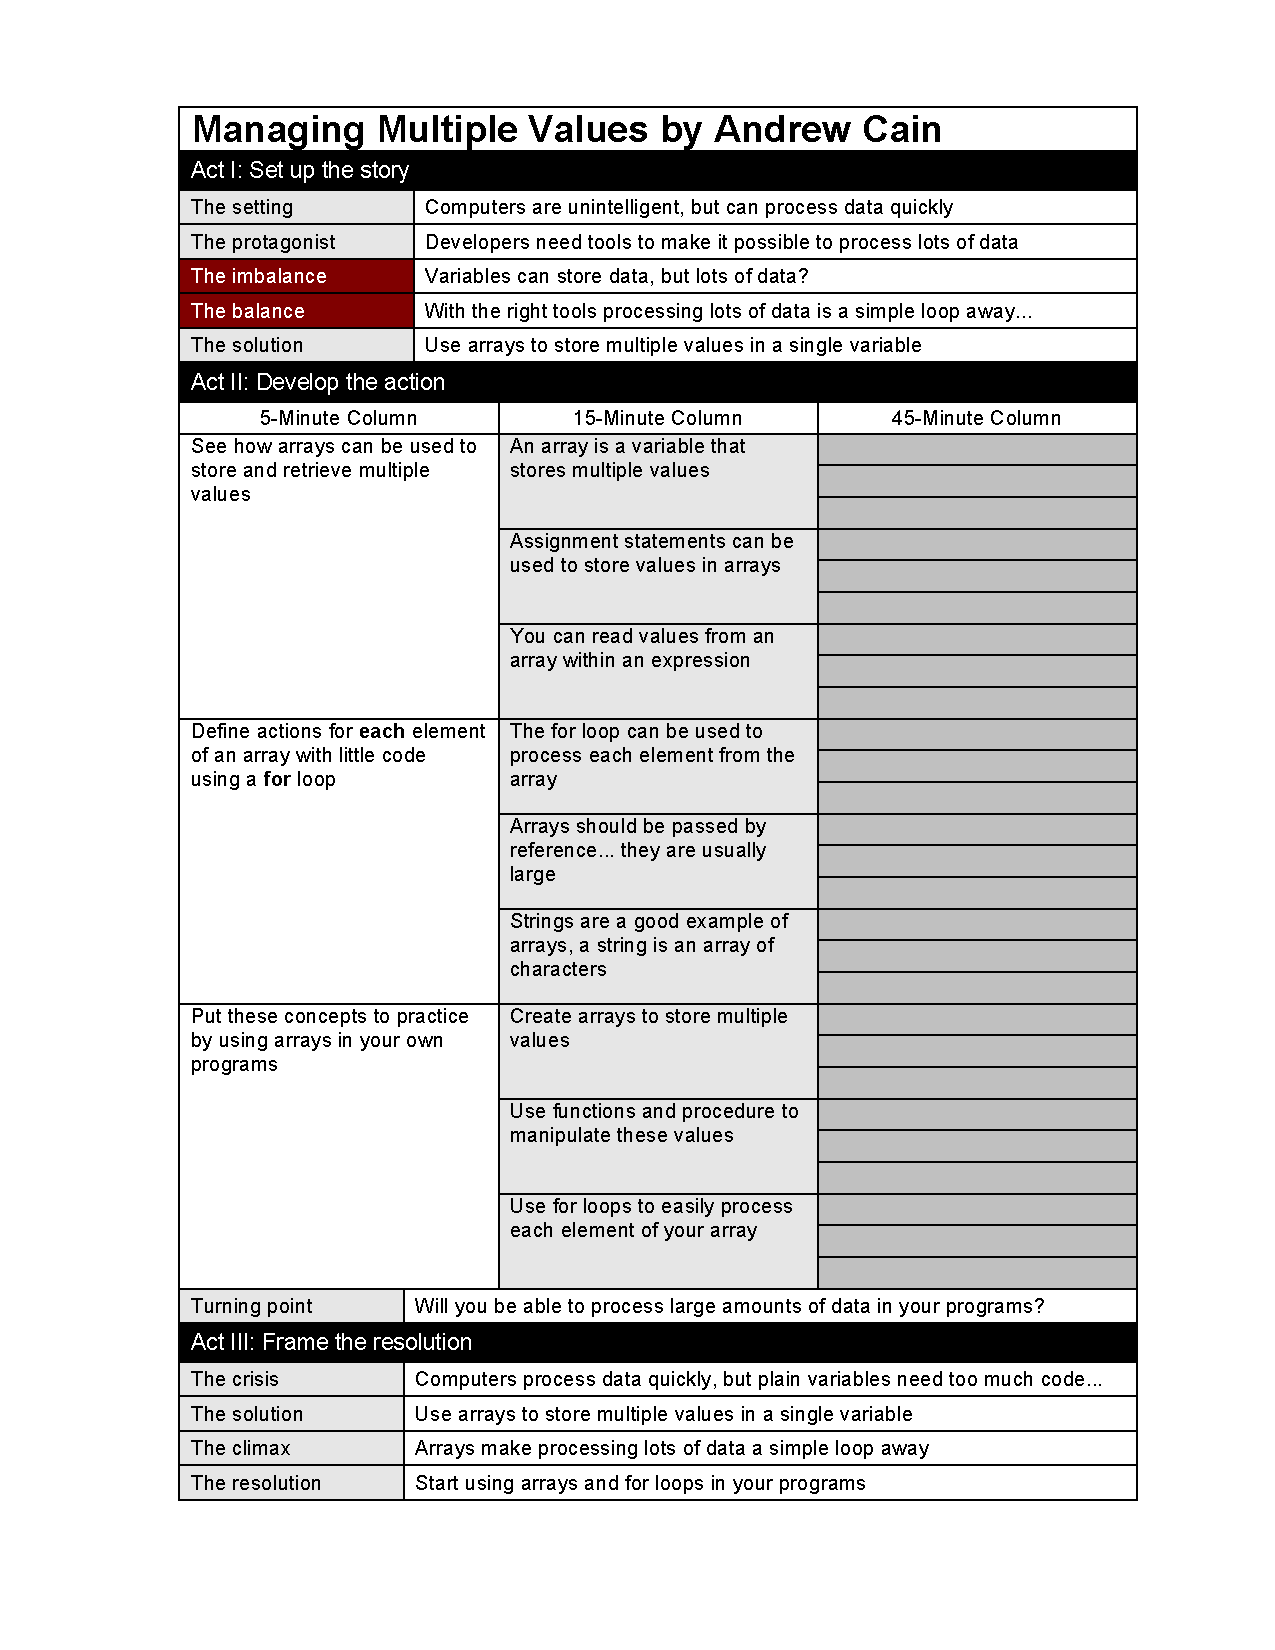
\includegraphics[width=\textwidth]{bbp}
	\caption{Example usage of the storyboard template, developed by \citet{Atkinson:2007} and available from \url{http://beyondbulletpoints.com}, that outlines the stages in a Beyond Bullet Points presentation.}
	\label{fig:bbp}
\end{figure}

The first five slides, termed Act 1, that set up the ``story'', telling the audience why they are there and centring them as the main character in the story. This helps motivate discussion, and focused teaching staff on clearly communicating the motivation behind the topic. The first five slides contain the following details:
\begin{enumerate}[label=Slide \arabic*:,labelwidth=*,align=left,noitemsep,nolistsep]
	\item \textbf{The setting}, sets the \emph{context}, positing the story at a relevant place within the content of the unit.
	\item \textbf{The protagonist} indicates the story is about the students, they are the focus not the teaching staff.
	\item Indicates \textbf{the imbalance}, stating a current problem, challenge or opportunity that motivates the need to find a solution.
	\item Juxtaposing the imbalance, \textbf{the balance} presents the goal, the situation in which the problem or challenge has been addressed, or the opportunity has been realised.
	\item Presents our \textbf{solution}, indicating how students (the protagonist) can get from the current \emph{imbalance} to the desired \emph{balance}.
\end{enumerate}

Slides contain a full sentence, written in an active voice. Ideally the slide text is accompanied by iconic visuals that set a theme or metaphor for the presentation. The time and resources necessary to prepare slides in this manner is, however, contrary to \pref{itm:agile}, being agile and willing to change these teaching and learning activities. If significant effort is spent developing slides in this way it is likely to increase resistance to change if adjustments to the topics message are desired. Instead, we suggest a minimalist approach with slides clearly showing the sentence text and using images to help communicate concepts central to the topic, as can be seen in the example slides shown in \fref{fig:lecture}.

For a fifteen minute presentation, the body of the presentation contained three main points, supported by three sub-points. Each addressed a ``why'' or ``how'' point, and supported the main solution. Once again these required a single short sentence in an active voice. The composition of these slides usually drew upon visuals created as part of the teaching and learning resources for the unit.

The last five slides conclude the presentation, reminding students of the overall solution and the new balance it brings about. These slides contain the following details:
\begin{enumerate}[noitemsep,nolistsep]
	\item The first slide in the conclusion was the \emph{turning point}. This is a question that asks a question of the students, indicating the presentation has turned to the conclusion. In effect it asks them if the concepts presented have shown them how to address the imbalance from the introduction.
	\item Next the \emph{crisis} slide restates the balance and imbalance, reminding the students of where the presentation started and where it was aiming to go.
	\item This then leads nicely to a restating of the \emph{solution}. This is an exact duplicate of the solution from the introduction, but now the student have been though the ``story'' and it should have more meaning.
	\item The \emph{climax} brings all of the pieces of the story together in summary and give the teaching staff a final opportunity to motivate students to study the topic further themselves.
	\item The final slide is the \emph{resolution}, and indicates the end of the presentation.
\end{enumerate}

Many of these guidelines from the Beyond Bullet Points approach were applied in the development of the lecture slides for the units discussed in \cref{cha:example_impl}. This included the general structure of the storyboard, though in some cases the three points were stretched to four but not beyond. The body of the presentations did include some information on ``what'' can be used, rather than purely focusing on ``how'' and ``why''. The use of active sentences, and visual communication, free from lists of bullet points, were also applied.

Focusing lecture slides in this manner helps to address the following principles from \cref{cha:guiding_principles}:

\begin{itemize}[noitemsep,nolistsep]
	\item Presentations aim to provide cognitive guidance, supporting students construction of knowledge. (\Pref{itm:construct})
 	\item Completing the story board requires a focus on the most important aspects for each topic. Where this focus is appropriately targeted, this also helps support alignment with intended learning outcomes. (\Pref{itm:align} and \Pref{itm:focus})
 	\item Shifting details from presentation to other resources requires a trust in students willingness to learn, supporting the need for a Theory Y attitude to motivation. (\Pref{itm:theory_y})
 	\item Using visuals for communicating core concepts, and minimalist themes for scaffolding slides, helps ensure presentations can be changed to respond to student needs. (\Pref{itm:agile})
 	\item The presentation style encourages a focus on concepts as little (if any) syntax would be used in the slides themselves. Instead, slides focus on visual representations to communicate programming concepts, leaving lower level details to be communicated via other means, as is discussed in \cref{cha:supporting}. (\Pref{itm:concepts})
 \end{itemize} 

\begin{figure}[htbp]
	\centering
	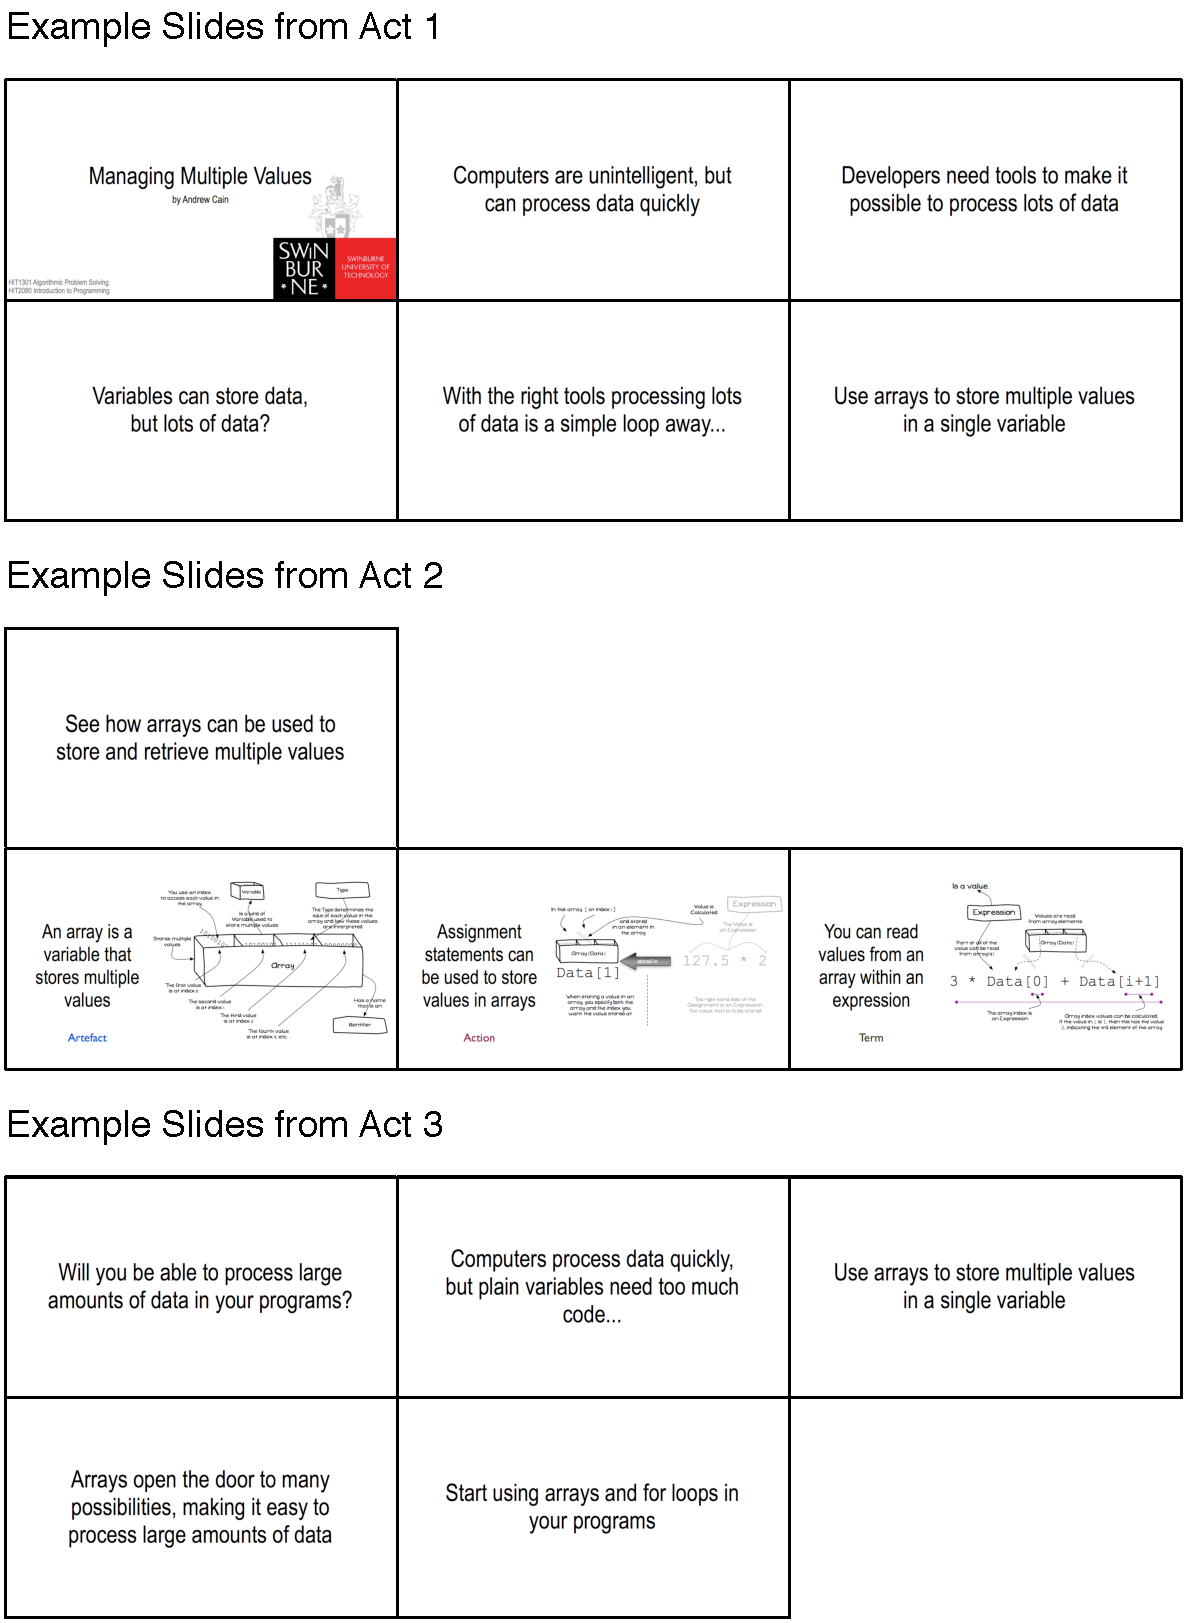
\includegraphics[width=\textwidth]{Lecture}
	\caption{Sample slides from the lecture created from the template shown in \fref{fig:bbp}. Act 1 and 3 use minimalist sentences, with visual representations of programming concepts being used to communicate the important concepts.}
	\label{fig:lecture}
\end{figure}

% subsubsection lectures (end)

\clearpage
\subsubsection{Interactive Lecture Demonstrations} % (fold)
\label{ssub:interactive_lecture_demonstrations}

Delivering one short, fifteen minute, presentation for each week's topic leaves a significant portion of a two hour lecture for other purposes. This time can be used to demonstrate the application of the concepts, providing students with a first experience of how these concepts can be used to create working programs. Similar approaches have been found to be an effective means of engaging students by \citet{Gaspar:2007} and \citet{Rubin:2013}.

The interactive sessions involve writing programs from scratch, guiding students through the whole software development process. This involves questioning students about what we should do, and which concepts we needed to apply. Program's are developed together with the students, enabling discussion as they evolve. This enables a focus on the thought processes behind program creation, taking students through the decisions that need to be made in crafting the design of the program being creating.

One important strategy we applied in these interactive coding sessions was for staff to become selectively forgetful, typically forgetting the syntax related to the current concept, for example. In this way, staff had to make use of the resources available to the students to \emph{find} the necessary details. For example, when focusing on how to declare variables this could be achieved by saying ``We want to create a variable here, but I can not remember the syntax. Where could I look to find the syntax for this?'' This triggers a discussion, and enables staff to demonstrate how to locate the associated resources, and lookup the relevant sections. Switching back to the code would be another point to ``forget'' the syntax, ``So what do I type first?''. The aim of this is to demonstrate to the students how these resources could be used to learn the language's syntax. In essence, providing an example of how to solve problems.

Depending on the topic, lectures typically follow one of two formats. Either the presentation was delivered in its entirety and was followed by the interactive session, or the interactive session was interwoven with the presentation itself. These two strategies can be applied at different times throughout the teaching period, depending on the topic. 

Topics in the first part of a unit are likely to have the interactive sessions interwoven with presentations. At this stage each of the concepts was totally new to the students. Presentations focused entirely on concepts is likely to make the topic very abstract. By interweaving live coding demonstration with presentations we aim to address student apprehension about how concepts are realised in practice.

Later topics, which reinforce earlier concepts, are likely to benefit from progressing more quickly through the slides and using a longer interactive demonstration. This would have the benefit of allowing a wider range of concepts to be demonstrated in a single session.

The use of interactive lecture demonstrations helps to address the following principles from \cref{cha:guiding_principles}:

\begin{itemize}[noitemsep,nolistsep]
	\item These sessions help provide students with a demonstration of applying unit concepts, aiding them in the construction of their own knowledge. (\Pref{itm:construct})
	\item In introductory programming, many of the intended learning outcomes relate to applying programming concepts to the development of small programs. These demonstrations are, therefore, directly aligned with activities we expect students to be able to demonstrate by the end of the unit.  (\Pref{itm:align})
	\item Guiding students through the use of supporting resources helps keep the focus on the most important concepts, while also helping students learn how to use available resources. (\Pref{itm:focus}, \Pref{itm:support} and \Pref{itm:concepts}).
	\item Demonstrations also provide an opportunity to illustrate good programming practice, and to show students examples of programs they are expected to be able to create. (\Pref{itm:expectations})
	\item Incorporating student input into the live demonstrations helps to motivate students, and requires a willingness to adapt to student requirements and needs. (\Pref{itm:theory_y} and \Pref{itm:agile})
\end{itemize}


% subsubsection interactive_lecture_demonstrations (end)

\clearpage
\subsubsection{Laboratory Sessions} % (fold)
\label{ssub:laboratory_sessions}

Laboratory sessions provide an opportunity for students to try applying the concepts covered in the lecture classes themselves. To help structure these sessions we organised these tasks into three groups: 

\begin{description}[noitemsep,nolistsep]
	\item [Laboratory tasks] were designed to be a guided exercise that was to be completed in class, providing detailed instructions on how to approach the problems presented.
	\item [Core tasks] had to be completed and submitted for feedback, helping students to develop pieces they can include in their portfolios.
	\item [Extension tasks] provided students with optional exercises they could use to extend themselves, requiring greater levels of independence and a better understanding of the concepts.
\end{description}

Tutors guide students through each week's laboratory tasks. These tasks were designed to give students their first hands-on experience with each week's concepts. Laboratory notes provided detailed step-by-step instructions to enable students to work through these on their own if they wanted, or need, to. At the end of the laboratory exercises students should be sufficiently prepared to undertake the core tasks.

Students then apply their understanding of each weeks concepts to complete the core tasks. It is important that these tasks ask the students to perform actions related to the unit's intended learning outcomes, as these tasks will help them create evidence they can include in their portfolios. For example, this could include tasks such as creating one, or more, small programs, or performing code reading exercises that ask students to hand execute programs and explain the program's behaviour, or identify issues in the presented code. 

Core tasks also form an integrated part of the formative feedback process. Once these tasks are completed students submit this work for feedback. Staff can then assess the work, and provide guidance on identified issues, and highlight possible misconceptions. If the work has issues, it can then be returned to the student with instructions on what needs to be corrected. Students can then work to address these issues, and associated misconceptions, and resubmit the work at a later stage. Where the task has been performed to a sufficient standard it can be signed off as complete, indicating that the student appears to have understood the associated concepts.

Extension tasks provide students with extra activities they can perform each week to demonstrate a deeper understanding of the associated concepts. These tasks are typically loosely defined, requiring students to explore the concepts in a more independent manner. A range of challenging tasks can be provided to support different student interests, and to provide students with ideas for activities that are likely to help them create pieces that will demonstrate valuable learning in their portfolios.

Laboratory sessions are highly student-centred, so organising these sessions in this way helps to address many of the principles from \cref{cha:guiding_principles}.  

\begin{itemize}[noitemsep,nolistsep]
	\item Activities help students develop their knowledge of the concepts being covered. (\Pref{itm:construct}) 
	\item Staff help ensure that these tasks relate to the unit's intended learning outcomes, ensuring students will be able to demonstrate how they have met these outcomes when they submit their portfolios. (\Pref{itm:align})
	\item Core tasks are used to provide students with formative feedback during the semester. (\Pref{itm:formative})
	\item Students are able to focus on the most important aspect for them at their current stage of development. Laboratory tasks focus on getting students started, core tasks focus on problems that demonstrate passable knowledge, while extension tasks can support the demonstration of more advanced levels of understanding. (\Pref{itm:focus})
	\item The formative process, with changes to core tasks being required before they are signed off, helps to clearly communicate the high standard expected of students. This is further supported by the list of extension tasks provided each week. These communicate the extra tasks the students \emph{should} be completing to demonstrate a deeper understanding of the concepts. (\Pref{itm:expectations})
	\item The different laboratory task levels each provide support for students at different stages of capability, while options in the extension tasks also help to support a range of student interests. (\Pref{itm:support})
	\item Using this approach students take a greater responsibility for their own learning. (\Pref{itm:theory_y})
\end{itemize}

% subsubsection laboratory_sessions (end)
% subsection content_approach (end)

\clearpage
\subsection{Summary} % (fold)
\label{sub:summary}

The overall strategy is defined by two approaches: the assessment approach, and the approach to content selection. Decisions related to these two approach were guided by the principles from \cref{cha:guiding_principles}, and resulted in the selection of a \textbf{portfolio assessment} approach to units that are taught using a range of student-centred teaching and learning activities. \fref{fig:overall_strategy} shows an updated version of \fref{fig:strategy}, showing the selected approaches discussed in this section. The next section describes the model for constructive alignment that developed from this overall strategy.

\begin{figure}[hb]
	\centering
	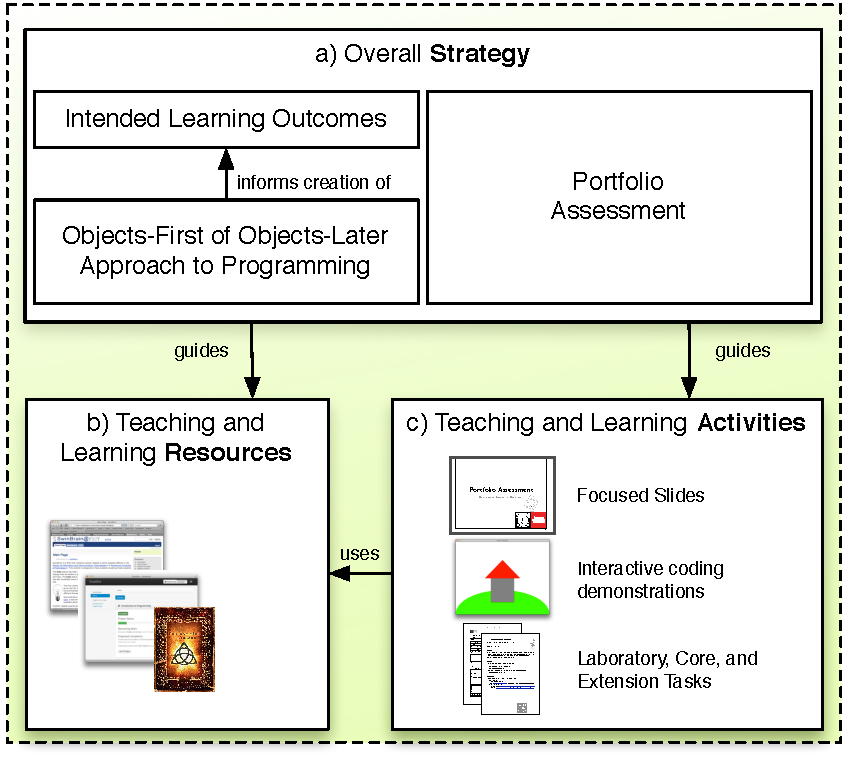
\includegraphics[width=0.8\textwidth]{OverallStrategy}
	\caption{An updated version of \fref{fig:strategy} showing the selected assessment approach, and the interactive teaching and learning activities.}
	\label{fig:overall_strategy}
\end{figure}

% subsection summary (end)
% section overall_strategy (end)
\clearpage
\section{Constructively Alignment with Portfolio Assessment} % (fold)
\label{sec:model}



\subsection{Model Overview} % (fold)
\label{sub:model_overview}

Having decided upon an overall strategy, the next stage of our research was to determine how Biggs' model of constructive alignment~\cite{Biggs:1996c}, and the details on using portfolio assessment suggested by \citet{Biggs:1997}, could be used to guide the creation of an introductory programming unit. This involved the examination of the practical advice from \citet{Biggs:2007}, which further elaborates on Biggs' model of constructive alignment and portfolio assessment. Using this together with the principles from \cref{cha:guiding_principles}, a model of constructive alignment for introductory programming was defined. The resulting model was documented in \citet{Cain:2012a}, and captured staff and student processes and the artefacts generated and exchanged throughout the learning process, as illustrated in \fref{fig:process_overview}.

\begin{figure}[htbp]
	\centering
	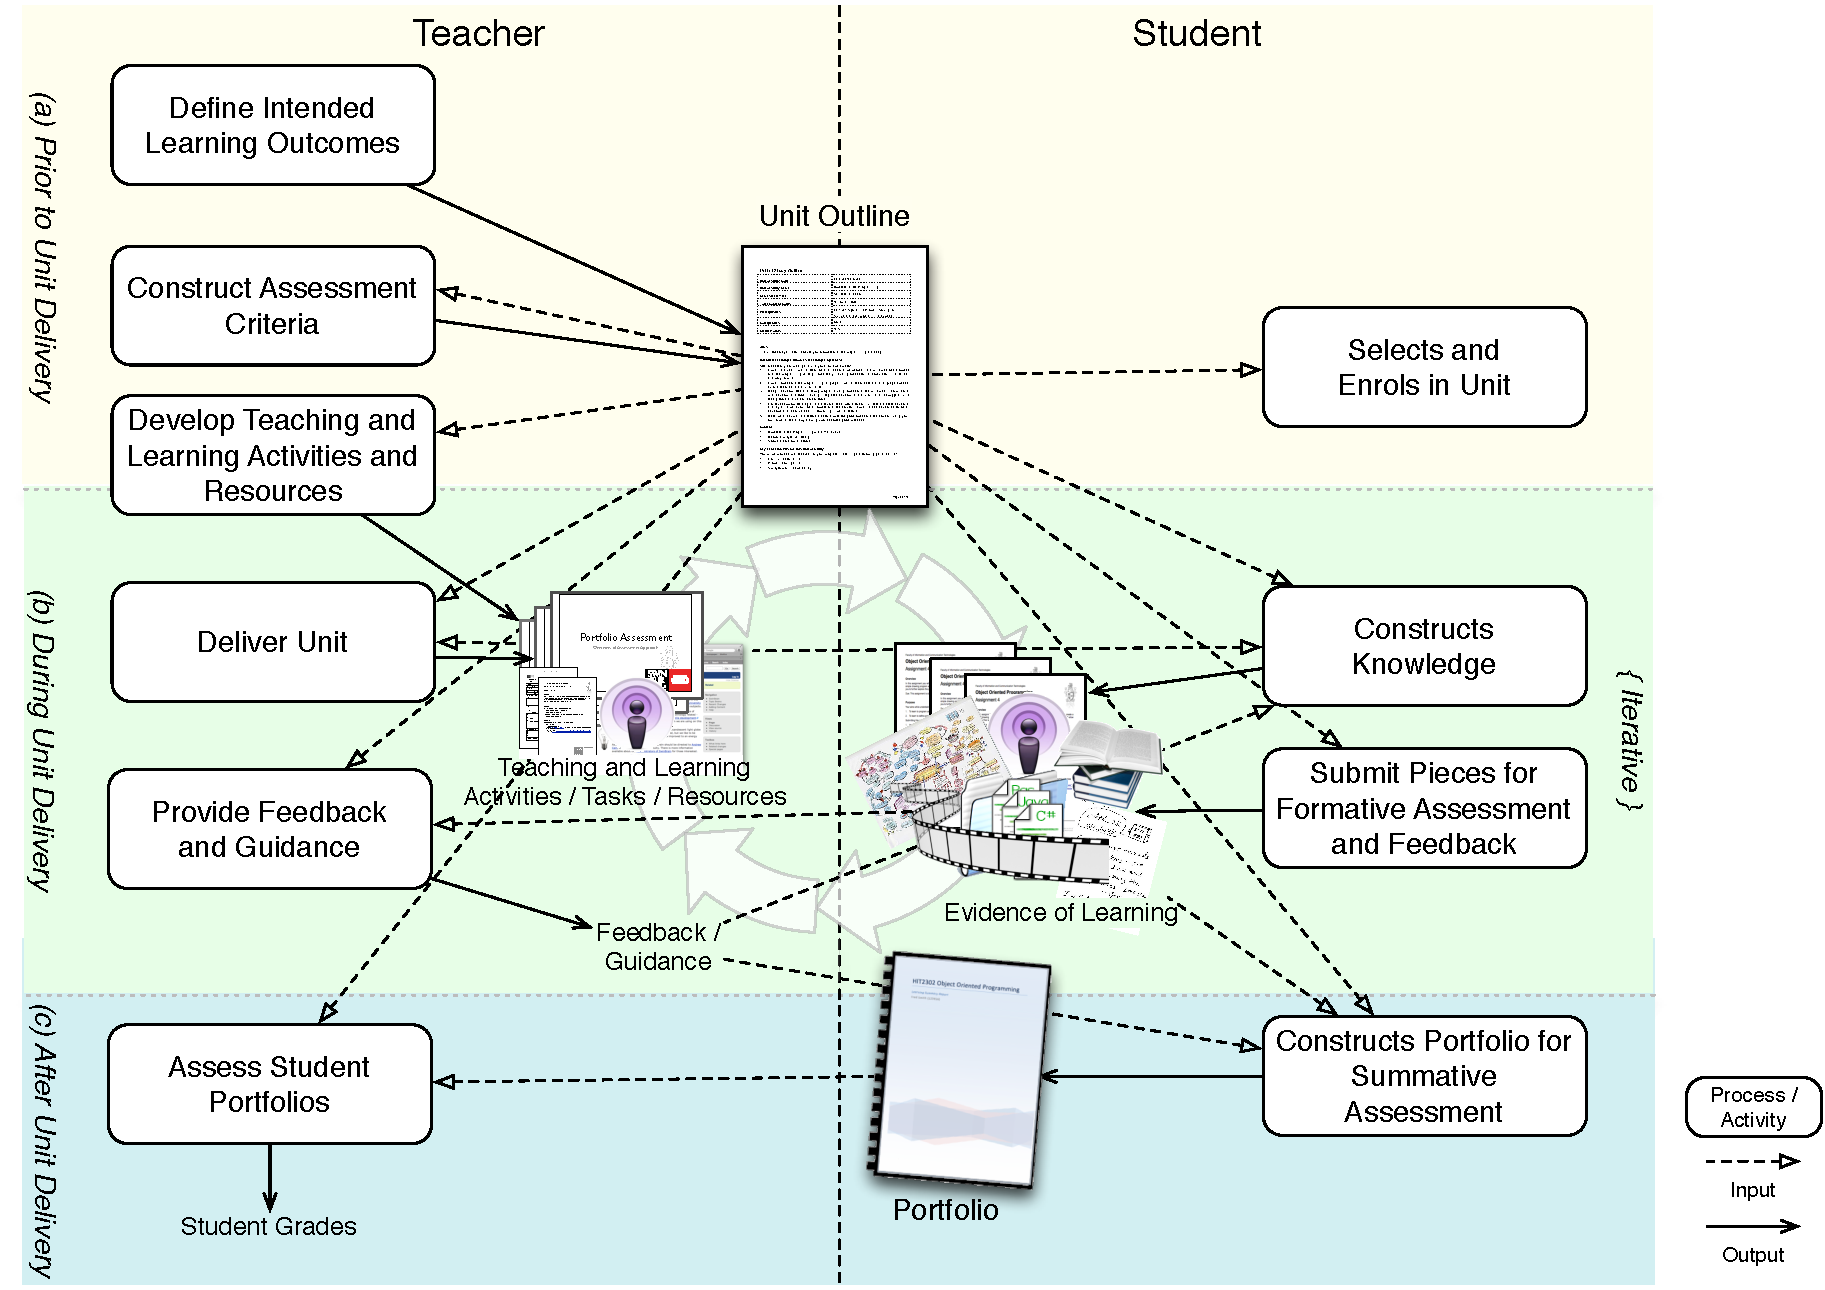
\includegraphics[width=\textwidth]{ProcessOverview}
	\caption{An overview of teacher and students roles (columns), and iterative delivery, in the constructive alignment model developed for the introductory programming units.}
	\label{fig:process_overview}
\end{figure}

Processes within the model are performed either by \emph{students} or \emph{teaching staff}. These processes are distributed across three stages of unit development and delivery: being either \emph{prior} to the start of the teaching period, \emph{during} the teaching period, or \emph{after} the teaching period. \fref{fig:process_overview} illustrates this with separate columns for teaching and student processes, and rows for the stages in which these processes occur.

Prior to the start of the teaching period (a) the teaching staff \emph{define intended learning outcomes} and \emph{construct assessment criteria}. Together these aspects form a critical component of unit, defining what students will be able to achieve after successfully completing the unit, and how well they must perform in order to achieve different grade outcomes. Both the intended learning outcomes and assessment criteria are documented in the Unit Outline, a document that is a common practice in university environments. The Unit Outline forms the central focus for subsequent processes, and informs and guides staff in the \emph{development of teaching and learning activities}. Unit outlines may also be used by students in evaluating units to select in their course of study.

The developed teaching and learning activities and their associated resources are then used during the teaching period (b) by staff to \emph{deliver the unit}. Students follow the guidance of teaching staff, and ideally these activities aid students as they \emph{construct knowledge}. The work that students produce can then be \emph{submitted for formative feedback}, which provides an opportunity for teaching staff to \emph{provide feedback and guidance}. The process of students undertaking activities, constructing knowledge, and receiving formative feedback is designed to be an ongoing iterative process throughout the teaching period.

After the conclusion of the teaching period (c) students prepare their work for summative assessment through the \emph{construction and submission of their portfolios}. These portfolios are then \emph{assessed by} the teaching staff against the intended learning outcomes and assessment criteria prepared prior to the unit's delivery.

Each of these processes is described in more detail in the following section.

% subsection model_overview (end)

\subsection{Processes within the Model} % (fold)
\label{sub:processes_within_the_model}

\subsubsection{Defining Intended Learning Outcomes} % (fold)
\label{sub:defining_intended_learning_outcomes}

Intended learning outcomes are central to the concept of constructive alignment as a statement of what students will be able to achieve at the end of the unit. Aligned curriculum in constructive alignment indicates that teaching and learning activities and assessment must \emph{align} to these intended learning outcomes. The findings in \cref{cha:background} indicate that alignment is typically performed by staff who indicate how teaching and learning activities and assessment tasks are aligned. Alignment is a matter external from the actual teaching itself. There is little involvement of the student in this process.

With portfolio assessment the alignment becomes intrinsically entwined with unit delivery and assessment. The teaching staff relinquish control of this aspect and the outcomes themselves take on their true purpose: as a statement of what students will be able to achieve at the end of the unit. All other aspects of the unit must now align to this purpose. Teaching and learning activities must prepare students to demonstrate that they have achieve these outcomes. Assessment aims to verify the extent to which students have reached these outcomes.

One way to conceptualise the central role of the intended learning outcomes is to picture this situation as a very long examination. The intended learning outcomes are the questions, the things students need to demonstrate they can do by the end of the ``exam''. The intended learning outcomes have become the assessment, a direct realisation of the fact that ``assessment always drives the curriculum'' \cite{Ramsden:2003}.  In this arrangement there is little opportunity for misalignment between the unit objectives and assessment, but a greater importance on the exact nature of the intended learning outcomes. This critical role of the intended learning outcomes means that they are instrumental in the success of the unit. 

For the introductory programming units it was important to design the intended learning outcomes so that, as a group, they cover the required programming competencies as well as the associated conceptual knowledge. The intended learning outcomes play a central role in driving the processes of both students and teaching staff. As a result, it is important they are expressed clearly and simply so as to be understood by all involved.

Development of unit outcomes has a variety of input sources. \citet{Thota:2010} propose inputs related to pedagogic theory (constructivism and phenomenography) as well as student factors such as approach to learning, learning styles, and prior knowledge. \citet{Armarego:2009} highlights the needs for inputs from industry, such as the Computer Science and Software Engineering Curriculum from professional standards bodies and associated Bodies of Knowledge \citet{Abran:2001}. For curriculum recommendations from professional standards bodies see \citet{Lethbridge:2006}, \citet{Cassel:2008}, and \citet{CSC2013}.

In defining the intended learning outcomes for an introductory programming unit using constructive alignment with portfolio assessment we suggest drawing upon these sources, as well as the guiding principles from \cref{cha:guiding_principles}, overall strategy, resourcing factors, and accreditation requirements as shown in \fref{fig:defining_ilos}. Resourcing factors provide additional constraints on what intended learning outcomes can include. Factors such as staffing, availability of texts, required tools, and others all need to be considered to ensure that students will be able to engage in activities associated with demonstrating the expected outcomes. Accreditation standards, such as the Australian Qualifications Framework \cite{AQF:2013}, require intended learning outcomes to demonstrate certain levels of achievement in order for degree programmes to gain recognition and funding. As these units will form an important part of programme objectives, these requirements must also be considered. 

\citet{Biggs:2007} provided a number of recommendations for the development of intended learning outcomes. They indicated that it was appropriate for a unit to have between four and six intended learning outcomes, expressed at suitably high cognitive levels. Adopting this approach enables the clear focus on what is important for the unit, and encourages depth over breadth, \pref{itm:focus} from \cref{cha:guiding_principles}. A small number of intended learning outcomes keep the focus clear for students.

% removed SOLO details from here...

As discussed in \cref{cha:background}, the SOLO Taxonomy proposed by \citet{Biggs:1982} provides a framework for ensuring intended learning outcomes aim for suitably high cognitive levels. Each of the identified cognitive levels has an associated list of verbs likely to elicit that level of activity. \tref{tbl:solo_verbs} lists selected verbs associated with the various levels of the SOLO taxonomy. These verbs can be used when defining the unit's intended learning outcomes. Biggs suggests that intended learning outcomes for university level units should aim for at least the multistructural level, with many units aiming for understanding at the relational level. In a review of science curricula in Danish universities, \citet{Brabrand:2009} argued that the SOLO taxonomy provided a good tool for specifying competency with a range of areas showing progressing depth in terms of SOLO verbs from undergraduate to graduate education.

\begin{figure}[p]
	\centering
	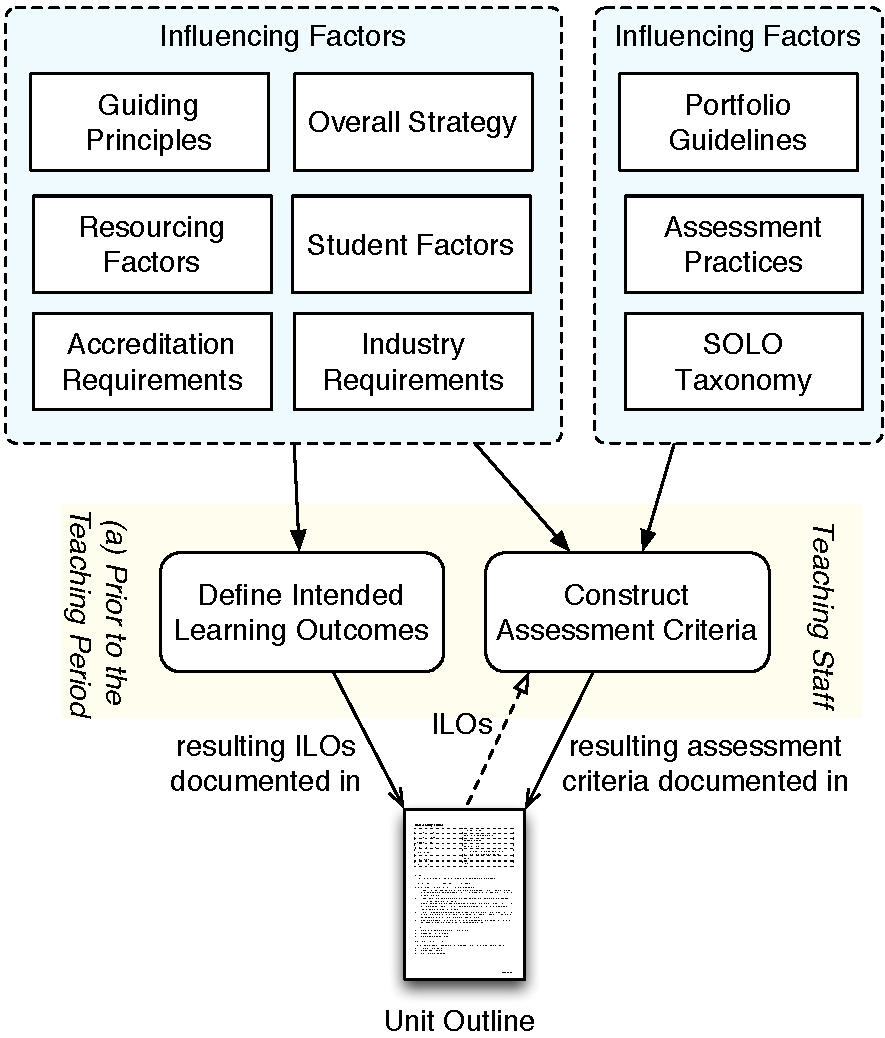
\includegraphics[width=0.55\textwidth]{DefiningILOs}
	\caption{Factors that influence the defining of a unit's intended learning outcomes, and the construction of assessment criteria. These activities are undertaken by teaching staff prior to the start of the teaching period, see (a) from \fref{fig:process_overview}. }
	\label{fig:defining_ilos}
\end{figure}

\begin{table}[p]
	\renewcommand{\arraystretch}{1.6}
	\centering

	\caption{Selected list of verb related to the levels of the SOLO Taxonomy suitable for defining intended learning outcomes, adapted from \citet{Biggs:2007}.}
 	\label{tbl:solo_verbs}
 	\footnotesize
    \begin{tabular}{lp{10cm}}
    SOLO Level        & Verbs likely to elicit indicated cognitive level \\
    \hline
    \textbf{Unistructural}     & memorize, identify, recognise, count, define, draw, find, label, match, name, quote, recall, recite, order, tell, write, imitate\\
    \textbf{Multistructural}   & classify, describe, list, report, discuss, illustrate, select, narrate, compute, sequence, outline, separate\\
    \textbf{Relational}        & apply, integrate, analyse, explain, predict, conclude, summarise, review, argue, transfer, plan, characterise, compare, contrast, differentiate, organise, debate, make a case, construct, review and rewrite, examine, translate, paraphrase, explain causes \\
    \textbf{Extended Abstract} & theorise, hypothesise, generalise, invent, originate, make original case\\
    \end{tabular}
\end{table}

We developed the following guidelines that can be used to inform the formation of the intended learning outcomes for portfolio assessed programming units.

%
% Can these "principles" be linked back to the Ch 3 ones??
% 
%
% I wonder about the use of "principle" in the context of both chapters?
% I wonder if the following (and in the following sections this chapter) could
% be renamed as something else e.g. guidelines?
% AC: renamed to guidelines
%
% Do you need/want to number these e.g.LO-1, LO-2 for "Learning Outcome guidelines"
% to refer to from Ch5 ??? 
%

\begin{itemize}[noitemsep,nolistsep]
  \item Express outcomes using verbs at an appropriate level of understanding with reference to the SOLO taxonomy.
  \item Cover both the required \emph{conceptual knowledge}, and \emph{programming competencies}.
  \item Use \emph{simple terms} (where possible) to communicate outcomes, thereby helping to ensure they can be understood by all students undertaking the unit.
  \item The number of outcomes should be \emph{minimal}, ideally between four and six. This is to help ensure that each outcome covers a meaningful body of knowledge to a sufficient depth.
  \item Outcomes need to be \emph{general} to facilitate assessment of diverse portfolios, and \emph{sufficient} to ensure that differing degrees of proficiency and understanding can be assessed.
  \item There needs to be \emph{flexibility} to enable students to choose a range of means when addressing outcomes.
\end{itemize}

Developing intended learning outcomes in this way helps to address the following principles from \cref{cha:guiding_principles}:
\begin{itemize}[noitemsep,nolistsep]
	\item Stated outcomes become the goal students work toward throughout the teaching period. Ensuring these are expressed using appropriate verbs from the SOLO taxonomy ensures they are likely to engage appropriate cognitive levels. (\Pref{itm:construct} and \Pref{itm:align})
	% \item (\Pref{itm:formative})
	\item Keeping the list of objectives short help ensure they are focused on the concepts related to the unit. (\Pref{itm:focus} and \Pref{itm:concepts})
	\item Using verbs from the relational level of the SOLO taxonomy helps communicate staff expectations. (\Pref{itm:expectations})
	\item Ensuring flexibility and clarity helps support a wider range of student interests and capabilities. (\Pref{itm:support})
	% \item (\Pref{itm:theory_y})
	% \item (\Pref{itm:agile})
	% \item (\Pref{itm:reflect})
	% \item (\Pref{itm:paradigm})
	% \item (\Pref{itm:authentic})
\end{itemize}





% subsection processes_within_the_model (end)
\subsubsection{Constructing Assessment Criteria} % (fold)
\label{sub:constructing_assessment_criteria}

Assessment criteria are developed alongside the definition of intended learning outcomes. The intended learning outcomes state what students need to demonstrate by the end of the unit, but these outcomes can be achieved to different standards. It is the role of the assessment criteria to state the required level of achievement students must demonstrate in order to be awarded various grade outcomes. This means that at the end of the teaching period students' portfolios can be assessed against the developed assessment criteria, but also that the assessment criteria can be used to guide the teaching and learning activities during delivery. Providing assessment criteria in the unit outline creates a simplified learning contract \cite{Stephenson:1993}, in which students know ``up front'' what is required to achieve the different grades. 

\pref{itm:formative} indicates that assessment should judge outcomes. To provide this holistic judgement the final summative assessment is \emph{criterion-referenced}, as suggested by \citet{Biggs:1997}. The criteria must, therefore, provide a means for teaching staff to assess submitted portfolios while also providing students with guidance they can use during the delivery and in the construction of their portfolios. Ensuring that the assessment criteria are stated clearly also helps ease students transition to this new form of assessment \cite{Smith:2001}.

There is some contention regarding the specification of assessment criteria for assessing portfolios. For example, some consider that by overly specifying criteria students are limited in what can be included (see \citet{Driessen:2005} and \citet{Tigelaar:2007}). However, \citet{Smith:2001} indicated that clearly communicating portfolio requirements helped ease students transition to this new, possibly unfamiliar, assessment approach. This is further supported by \citet{Allan:1996}, who argued that clear communication of intended learning outcomes and assessment criteria enabled students to focus on developing knowledge required to succeed in a unit, and by \citet{Thorpe:2000} who noted that students found it easier to reflect on their learning if they were able to apply criteria defined by teaching staff.

The assessment criteria development process takes input from the intended learning outcomes, along with guidelines for portfolio assessment \cite{Biggs:2007} and levels of achievement from the SOLO taxonomy \cite{Biggs:1982} as shown in \fref{fig:defining_ilos}. The resulting criteria are placed alongside the intended learning outcomes in the unit outline.

In order to facilitate assessment, and to guide student activity, the assessment criteria need to indicate clearly distinct requirements for each grade outcome. In the university where this work was carried out there are five grade categories: Fail, Pass, Credit, Distinction and High Distinction. The assessment criteria indicate what students need to demonstrate to achieve each grade. 

The following list presents the assessment criteria developed in this work. The criteria are cumulative, with each level beyond pass requiring all previous requirements to be satisfied in addition to some deeper level of understanding being demonstrated. Pass requires that each intended learning outcome is met to a minimally acceptable standard, which will depend on the verb used in their description. Credit then requires an overall picture of the unit, with students starting to see how the various aspects of the unit come together as a whole. This is then required to achieve the Distinction grade, in which students must show they can apply unit concepts to the creation of a piece of work of their own invention. This does not need to be new or ``ground breaking'' work, just something the student created on their own that shows all of the intended learning outcomes in play. High Distinction then goes beyond this by asking students to engage is a small research project, encouraging them to work toward an extended abstract\footnote{Extended abstract requires a level of understanding where new knowledge can be created.} level of understanding, but not requiring that they achieve this.
\begin{description}[noitemsep,nolistsep]
	\item[Fail] is a result of anything less than Pass level.
	\item[Pass] demonstrates \emph{minimally acceptable} level of achievement. Students have been able to complete core tasks from the teaching and learning activities, and pass any hurdle\footnote{Hurdle requirements are anything that must be ``passed'' to pass the unit, but do not contribute marks toward the final grade.} requirements.
	\item[Credit] demonstrates all Pass requirements and shows a \emph{good} depth of understanding across all intended learning outcomes, but does not go beyond presented work. Demonstrates at least a multistructural level of understanding of the unit overall.
	\item[Distinction] demonstrates Credit level requirements and the ability to \emph{apply} unit concepts to the creation of work of the students own invention. This demonstrates at least a relational level of understanding of the unit overall.
	\item[High Distinction] demonstrates all Distinction level requirements and the ability to \emph{research} a topic related to the unit. This still requires only a relational level of understanding, but provides opportunities and encouragement for students to explore beyond the current knowledge and work toward that extended abstract level of understanding.
\end{description}

\clearpage 

The following guidelines were used to inform the definition and communication of the assessment criteria:

%
% Can these "principles" be linked back to the Ch 3 ones??
% 

\begin{itemize}[noitemsep,nolistsep]
  \item Communicate assessment criteria using \emph{simple terms} (as suggested for the outcomes).
  \item Require sufficient progress to be demonstrated for all intended learning outcomes. At least a multistructural level of understanding should be obtained for passing students.
  \item Higher grades should require:
  \begin{itemize}[noitemsep,nolistsep]
  	\item evidence of \emph{deeper learning}, while specifically avoiding an excessive volume of work.
  	\item integrated understanding across related intended learning outcomes, as well as within each intended learning outcome.
  \end{itemize}
  \item Aim to develop \emph{clearly distinct} assessment criteria for each grade outcome, facilitating timely assessment and providing clear requirements for students.  
  \item Clearly \emph{map assessment criteria} to grade outcomes, ensuring students and staff have a shared understanding of how a portfolio relates to final grades.
\end{itemize}

Constructing the assessment criteria using these guidelines helps to address the following principles from \cref{cha:guiding_principles}:

\begin{itemize}[noitemsep,nolistsep]
	\item Requiring progressively higher levels of understanding for each grade classification help promote deep learning, and indicates staff expectations in terms of required levels of demonstration. (\Pref{itm:construct} and \Pref{itm:expectations})
	\item Assessment criteria align to unit outcomes, with higher grades requiring students to demonstrate an understanding of the relationships between the intended learning outcomes and their associated concepts. (\Pref{itm:align} and \Pref{itm:concepts})
	\item Grades are awarded using criterion referenced assessment, assessing students' learning outcomes. (\Pref{itm:formative})
	\item Specific criteria help focus students on the most important aspects, with higher grades requiring demonstration of deeper learning. (\Pref{itm:focus})
	\item The use of simple terms help support a wide range of student language capabilities. (\Pref{itm:support})
	\item Students can take responsibility for their learning, being able to aspire to achieve a given grade, and being able to apply their own imagination and interests in applying concepts to achieve higher grades. (\Pref{itm:theory_y})
	\item Evidence from student submissions provide a source of evidence for change, and can be reflected upon at the end of each teaching period to inform future changes. (\Pref{itm:agile} and \Pref{itm:reflect})
	% \item (\Pref{itm:paradigm})
	% \item (\Pref{itm:authentic})
\end{itemize}



% section a_constructively_aligned_model_for_introductory_programming (end)

\clearpage
\subsubsection{Develop Teaching and Learning Activities and Resources} % (fold)
\label{ssub:develop_teaching_and_learning_activities_and_resources}

Having defined the intended learning outcome, and assessment criteria, teaching staff develop, or select, appropriate teaching and learning activities and resources. \fref{fig:develop_tlar} illustrates the role of this process in the overall unit delivery. The process uses inputs from the Unit Outline, and generates both teaching and learning activities and resources.

\begin{figure}[htbp]
	\centering
	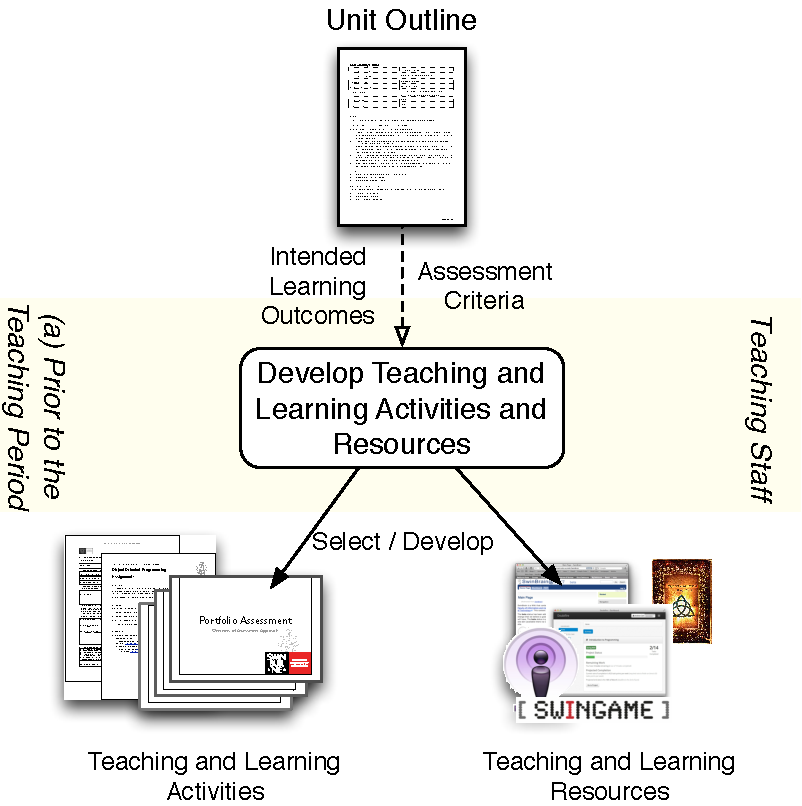
\includegraphics[width=0.6\textwidth]{DevelopTLAR}
	\caption{Development of teaching and learning activities and resources uses details from the unit outline to create/select appropriate resources and activities to ensure students engage appropriate activities during the teaching period.}
	\label{fig:develop_tlar}
\end{figure}

The teaching and learning activities aim to elicit appropriate behaviour from students, ensuring that they engage in the cognitive processes representative of the desired level of achievement for each intended learning outcome. Output generated from this process includes lecture slides and tutorial/laboratory handouts. In relation to the overall strategy, these activities are likely to change frequently as teaching staff become better able to direct student efforts. In keeping with our agile principles (\pref{itm:agile}) the effort spent on developing these teaching and learning activities should be minimised.

In contrast, teaching and learning resources provide students with detailed information they will require to successfully complete the teaching and learning activities. If designed appropriately, these resources should have a longer lasting value, and can change less frequently than the teaching and learning activities. Central to this approach is the idea of focusing (\pref{itm:focus}) each aspect of the teaching and learning environment to best benefit the construction of student knowledge (\pref{itm:construct}). Teaching and learning resources provide details, and extra attention and effort are required in their development, with the benefit of being able to be used in a range of contexts. Examples of resources include textual and visual illustrations, video podcasts showing example usage, online tools, and supportive software. Some of these resources can then be used in the creation of the lecture slides, but the lectures focus on providing cognitive guidance, directing students through the most important aspects with the details to be discovered later when students make use of the provided resources.

%
%Can these "principles" be linked back to the Ch 3 ones??
% 

The following guidelines were used to inform this process:

\begin{itemize}[noitemsep,nolistsep]
	\item Teaching and learning \textbf{activities} should:
	\begin{itemize}[noitemsep,nolistsep]
	 	\item Actively engage the students.
	 	\item Align with the unit's intended learning outcomes.
	 	\item Focus on providing guidance:
	 	\begin{itemize}[noitemsep,nolistsep]
		 	\item Lectures should inform, motivate and inspire students. Providing students with the key ingredients needed to get started with the tutorial/laboratory tasks.
		 	\item Tutorial/Laboratory tasks should direct students to perform activities that engage appropriate cognitive levels, helping them create artefacts that can be included in their portfolios.
	 	\end{itemize}
	 \end{itemize} 

	\item Teaching and learning \textbf{resources} should:
	\begin{itemize}[noitemsep,nolistsep]
		\item Provide the details students require to perform the tasks from the teaching and learning activities.
		\item Be created with a focus on re-usability.
		\item Support a range of different learning styles.
	\end{itemize}
\end{itemize}

Material developed using these guidelines address the following principles from \cref{cha:guiding_principles}:

\begin{itemize}[noitemsep,nolistsep]
	\item Aligning activities to intended learning outcomes ensures students develop appropriate knowledge related to the units concepts. (\Pref{itm:construct}, \Pref{itm:align}, and \Pref{itm:concepts})
	% \item (\Pref{itm:formative})
	\item Focusing these activities on appropriate cognitive levels helps direct student attention, and communicate staff expectations. (\Pref{itm:focus} and \Pref{itm:expectations})
	% \item (\Pref{itm:support})
	% \item (\Pref{itm:theory_y})
	\item Separating activities from resources helps enable activities to change. (\Pref{itm:agile})
	% \item (\Pref{itm:reflect})
	% \item (\Pref{itm:paradigm})
	% \item (\Pref{itm:authentic})
\end{itemize}

See \sref{sub:delivery_approach} for some example activities developed using these guidelines.


% subsubsection develop_teaching_and_learning_activities_and_resources (end)

\subsubsection{Iteratively Deliver Unit and Provide Feedback} % (fold)
\label{ssub:deliver_unit}

Constructive learning theories emphasise the active role of the learner in constructing knowledge. Our guiding principles are centred on this notion and adopt Biggs' pragmatic view of constructivism. The iterative, students centred, delivery process aims to embody Biggs' quote ``It's what the student does that counts.'' \cite{Biggs:1996c}, a statement that can be traced back to Tyler's quote, ``It is what he does that he learns, not what the teacher does'' \cite{Tyler:1969}.

Existing work on constructive approaches to teaching introductory programming provide some advice on designing and delivering student-centred teaching and learning activities. \citet{BenAri:1998,BenAri:2001} discussed the need for students to construct appropriate models of the computer. \citet{VanGorp:2001} described collaborative and constructive environments with the use of code walk-throughs, writing code, debugging and other activities. \citet{Thramboulidis:2003} presented a design-first approach to object oriented programming that focused on engaging students with object oriented design processes. \citet{Wulf:2005} reported strategies such as moving content from lectures to online video presentations. Similarly, the work of \citet{Thota:2010} also presented constructive approaches to teaching introductory programming that focused on group work, and the active role of the student.

\begin{figure}[p]
	\centering
	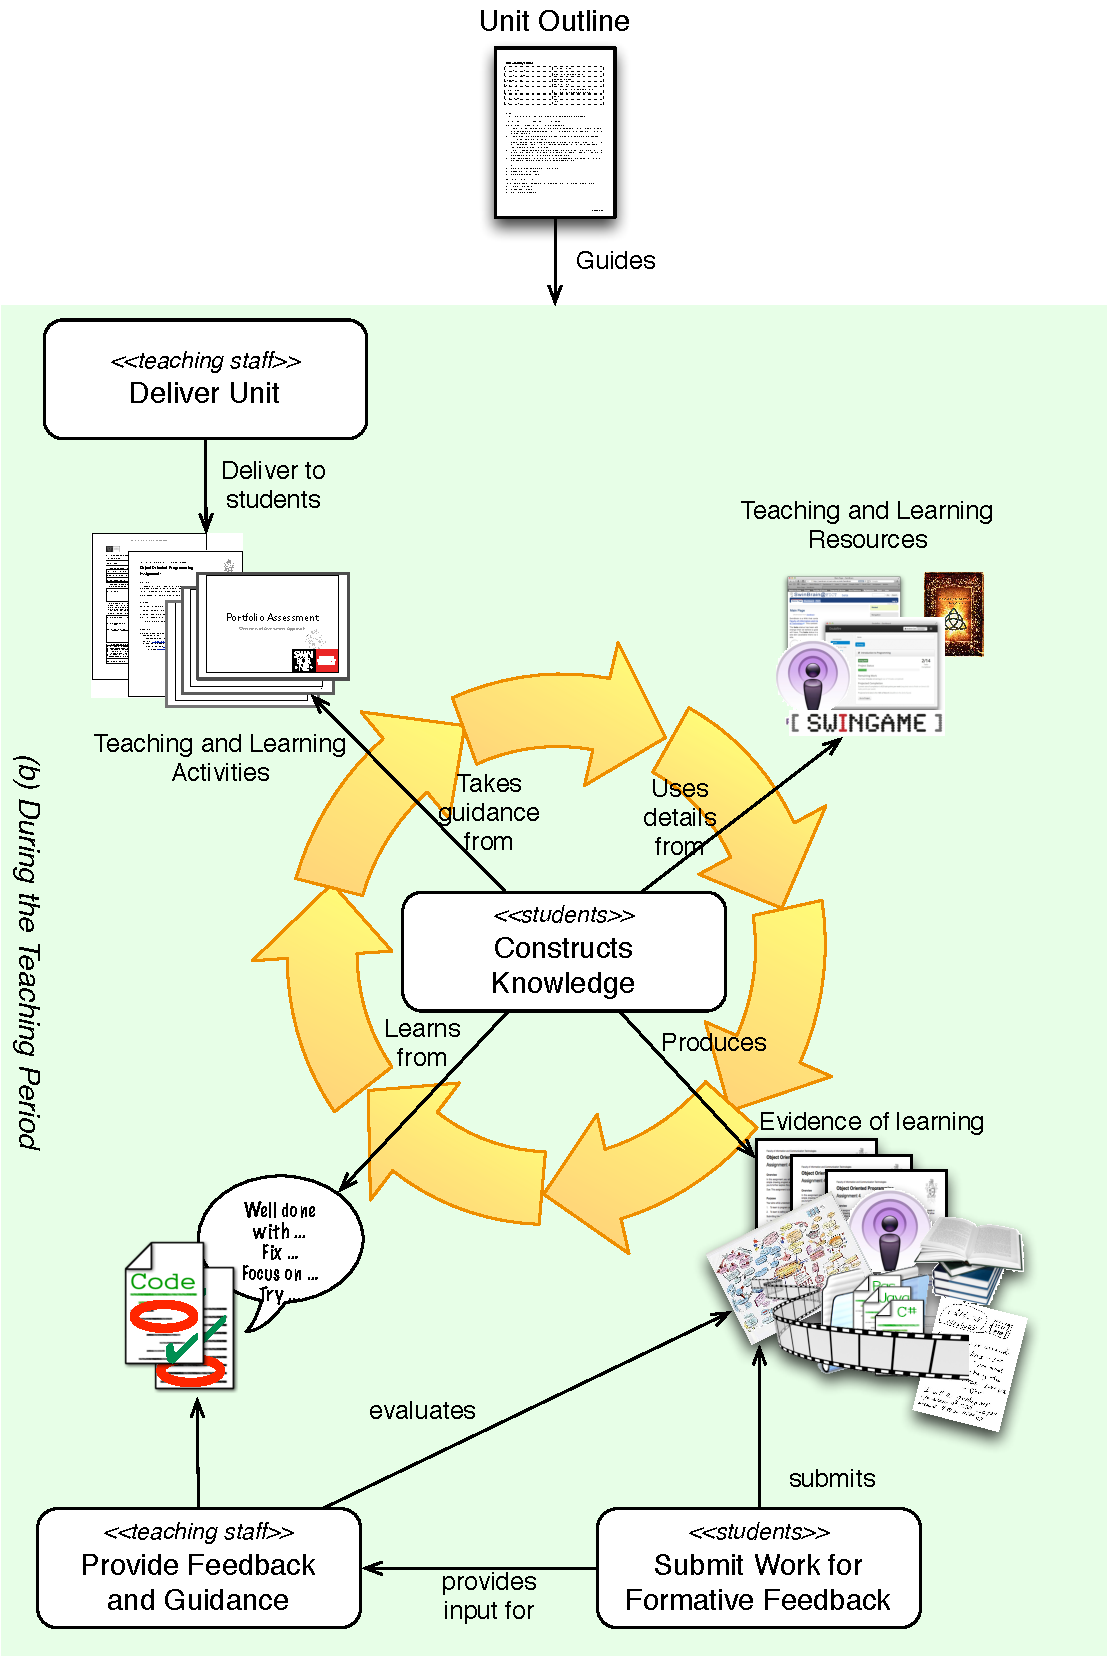
\includegraphics[width=0.8\textwidth]{DeliverUnit}
	\caption{Iterative nature of the unit delivery process}
	\label{fig:deliver_unit}
\end{figure}

\fref{fig:deliver_unit} illustrates the iterative delivery process at the heart of the model presented. The process centres on the students construction of knowledge, which draws up the teaching and learning activities and resources. This active process of learning generates pieces of work that the student submits for formative feedback. The teaching staff evaluate the evidence presented, trying to identify issues with the students current mental models, and provide formative feedback to the student. This feedback helps inform the student of their progress, and provides them with tasks they can act up thereby ensuring we close the loop.

All of these processes occur on a weekly basis, with rapid iteration ensuring feedback is timely and gives students the best chance of addressing misconceptions before the end of the teaching period. Each week, students will:

\begin{enumerate}[noitemsep,nolistsep]
	\item Attend lectures which guide them in relation to key aspects and motivations.
	\item Undertake set tasks from tutorial handouts, while drawing upon teaching and learning resources for required details.
	\item Produce work and submit for feedback.
	\item Receive feedback aimed to help them improve, and a list of changes required to meet the expected standard.
\end{enumerate}

For any one topic, this iterative process may take a couple of iterations before the student is successful in getting the work signed off. \fref{fig:construct_knowledge} is an illustration shown to students to indicate the iterative nature of the submission process. The highly connected nature of the topics in introductory programming means that it is critical students understand earlier topics before they move on. Work that is submitted is not considered complete by teaching staff until it demonstrates certain levels of understanding. While this is not the case, students need to correct and resubmit the work.

\begin{figure}[p]
	\centering
	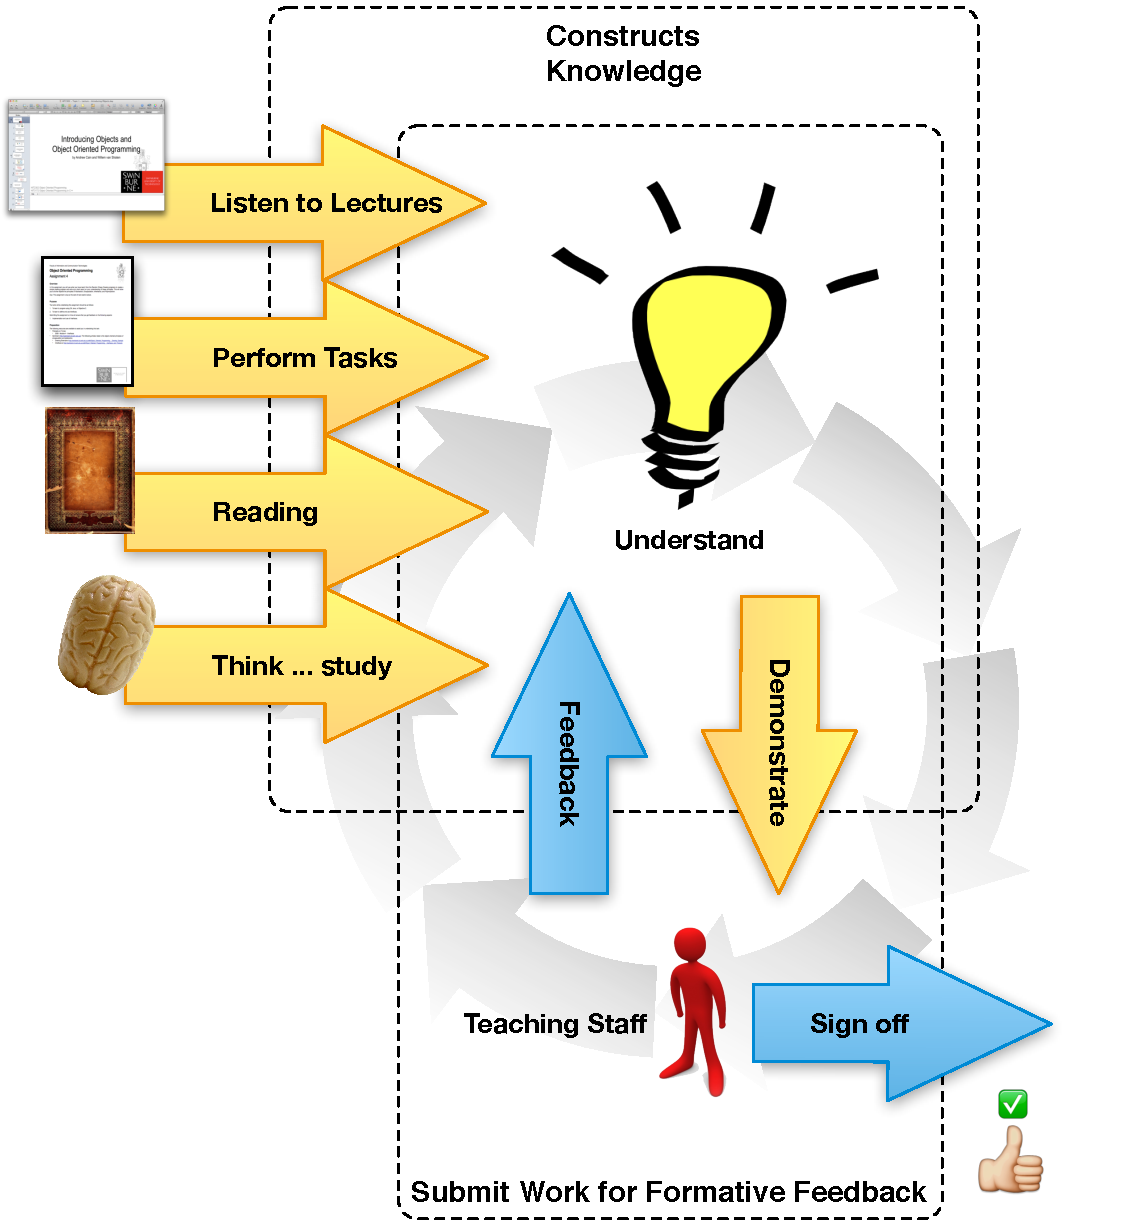
\includegraphics[width=0.9\textwidth]{ConstructKnowledge}
	\caption{Iterative process students undertake to get work signed off.}
	\label{fig:construct_knowledge}
\end{figure}

Requiring students to resubmit work ensures that no topic is half done. This focus on quality, and depth of understanding, helps communicate the high standards expected of students, \pref{itm:expectations}. Students are expected to submit some work for assessment each week. To enable fast turn around, this work is required in hard copy at the start of each week's lecture. This work is then evaluated by the teaching staff \emph{before} that week's tutorial classes (in practice 1 to 2 days). In the tutorial classes the work is returned to students, and the teaching staff briefly discuss progress with each student and the aspects of their work they can improve upon. This dialogue focuses on the student's individual understanding, and their demonstration thereof.

The following guidelines were developed and used to inform the planning and delivery of teaching and learning activities:

%
% Can these "principles" be linked back to the Ch 3 ones??
% 

\begin{itemize}[noitemsep,nolistsep]
  \item Provide opportunities through activity design to actively engage students -- \emph{it is what the student does that counts}.  
  \item Relate all activities to the objectives, providing students with opportunities to create evidence for their portfolio.
  \item Use ungraded formative feedback to aid knowledge construction, with preference for small, frequent guidance.
\end{itemize}

Adopting these guidelines in the delivery of a unit will help address the following principles from \cref{cha:guiding_principles}:

\begin{itemize}[noitemsep,nolistsep]
	\item Frequent formative feedback aids students' construction of knowledge, and helps ensure learning aligns with unit outcomes and concepts. (\Pref{itm:construct}, \Pref{itm:align}, \Pref{itm:formative} and \Pref{itm:concepts})
	\item Feedback can focus on the most important aspects, ensuring it is relevant to each student and their current level of understanding. (\Pref{itm:focus} and \Pref{itm:agile})
	\item Requiring work to be completed to a good standard helps reinforce staff expectations, and supports students by encouraging reflection and deep approaches to learning. (\Pref{itm:expectations}, \Pref{itm:support}, and \Pref{itm:reflect})
	\item Using formative feedback, without the marks associated with summative assessment, requires a Theory Y attitude to student motivation. (\Pref{itm:theory_y})
	% \item (\Pref{itm:paradigm})
	% \item (\Pref{itm:concepts})
	% \item (\Pref{itm:authentic})
\end{itemize}

% subsubsection deliver_unit (end)

\subsubsection{Construction, Submission, and Assessment of Portfolios} % (fold)
\label{ssub:construction_submission_and_assessment_of_portfolios}

The final phase of the process is the development and submission of portfolios by students, and assessment by staff. This process uses the intended learning outcomes and assessment criteria from the Unit Outline to determine what needs to be demonstrated and assessed. \fref{fig:portfolio_processes} illustrates the processes for portfolio construction by students, and assessment by staff. Students construct their portfolios from work completed during the teaching period. This work can incorporate feedback received, enabling students to showing off their best work and providing them with encouragement to act upon the feedback. \fref{fig:portfolio_pieces} shows an illustration used to explain the portfolio construction process to students. 

In preparing the portfolio, students must demonstrate that they have met all of the unit's intended learning outcomes. This alignment is documented by students in a \emph{Learning Summary Report}. The Learning Summary Report starts with a self assessment, in which the student indicates which grade they are \emph{applying} for with this portfolio. In the following sections students provide justification for why they should be awarded this grade. Students are required to list the pieces of work they have includes, and then explain how these pieces demonstrate that the student has attained all intended learning outcomes. The report ends with a reflection in which the student is encouraged to reflect upon the significance of what they have learnt, as well as on the process of learning itself. This learning summary report is then combined with the other pieces of work, printed, bound and submitted for assessment.

\begin{figure}[p]
	\centering
	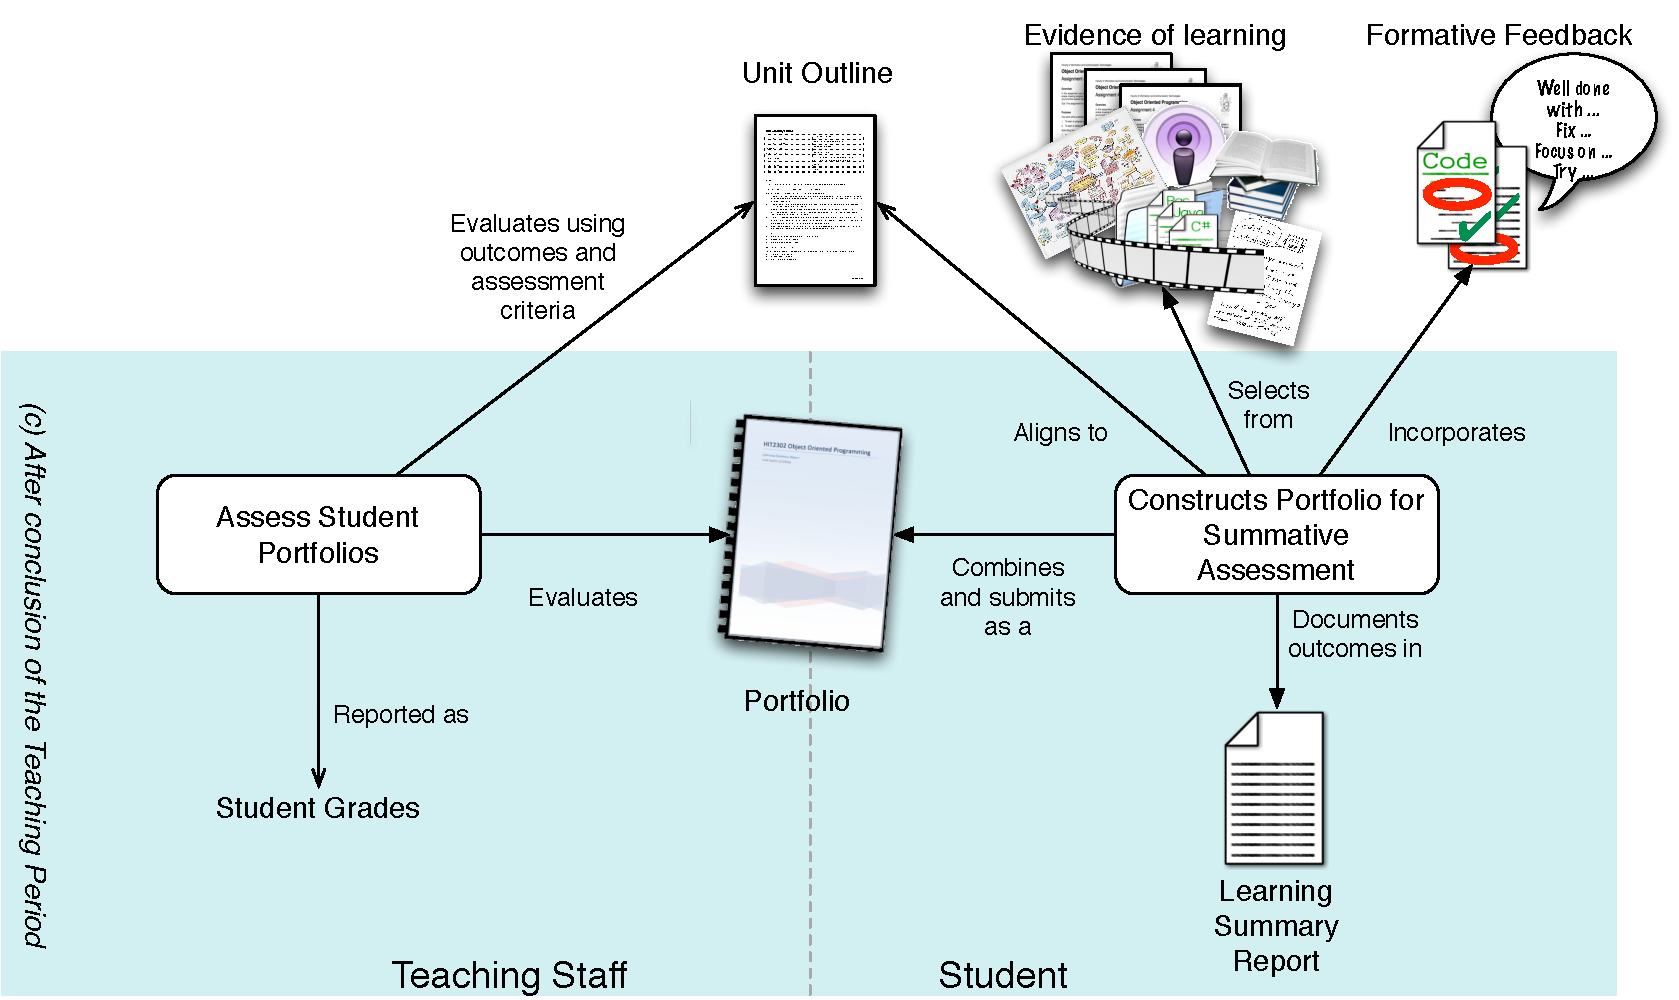
\includegraphics[width=\textwidth]{PortfolioConstructionAssessment}
	\caption{Processes of constructing, submitting, and assessment portfolios.}
	\label{fig:portfolio_processes}
\end{figure}

\begin{figure}[p]
	\centering
	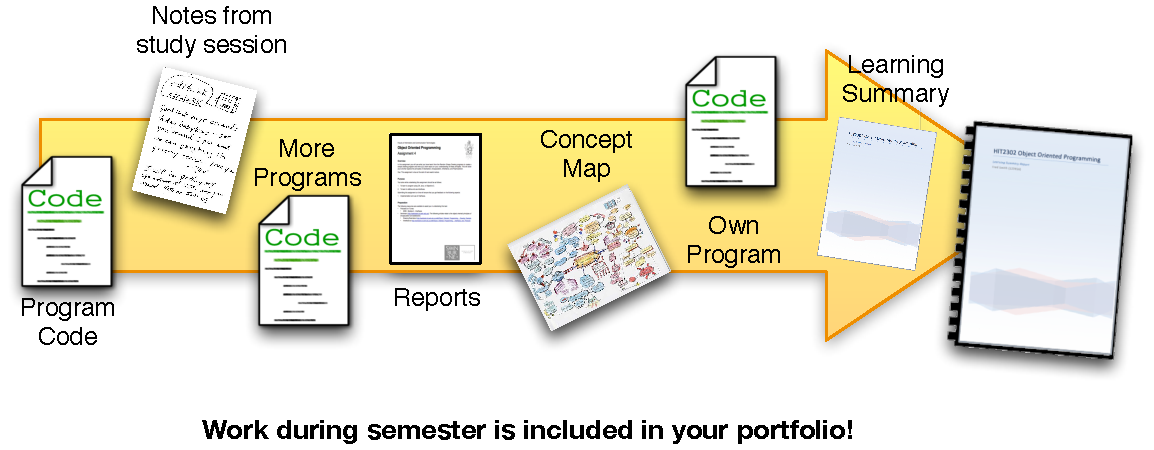
\includegraphics[width=0.9\textwidth]{PortfolioPieces}
	\caption{Illustration shown to students to highlight the process of constructing their portfolio during the teaching period}
	\label{fig:portfolio_pieces}
\end{figure}

The submission process differs based upon the grade students are aiming for in their portfolios. Students aiming for a Pass or Credit grade submit their portfolio by a set date in the examination period. These portfolios contain primarily work set out in the teaching and learning activities (``core'' tasks), and will have been checked already by teaching staff throughout the teaching period as part of the formative feedback process. Students aiming for Distinction or High Distinction are required to present their portfolio at an interview. In this interview students outline their custom work, and discuss how this relates to the unit's intended learning outcomes. The interviews are conducted in an open, relaxed, and friendly manner, and students are encouraged to elaborate on what they have achieved.

\clearpage
Based on our experience we suggest the following guidelines be used to inform the creation and assessment of portfolios:

%
% Can these "principles" be linked back to the Ch 3 ones??
% 

\begin{itemize}[noitemsep,nolistsep]
  \item Encourage unique, diverse, concise, and strongly aligned evidence.
  \item Motivate students to include evidence of learning from formative experience.
  \item Accurately and consistently follow the terms of the assessment criteria, as this is the \emph{contract} the students work towards.
  \item Require students to reflect on their learning, and the evidence in their final portfolio, with respect to the intended learning outcomes of the unit and the assessment criteria.
  \item Use an interview, or hurdle test(s), to check for minimal pass criteria in an invigilated manner. Where tests are used they need only distinguish between Pass and Fail, and do not need to address higher grades. 
\end{itemize}

Applying these guidelines to the creation and assessment of portfolios helps address the following principles from \cref{cha:guiding_principles}:

\begin{itemize}[noitemsep,nolistsep]
	\item Students are actively encouraged to include pieces that demonstrate their learning.  (\Pref{itm:construct})
	\item Pieces included in the portfolio must align with the unit's intended learning outcomes. (\Pref{itm:align})
	\item Feedback from the formative feedback process can be acted upon by students, with improved versions of earlier work being included as pieces in their final portfolios. (\Pref{itm:formative})
	% \item (\Pref{itm:focus})
	\item In writing the Learning Summary Report, students need to address the assessment criteria that capture staff expectations for each grade outcome. (\Pref{itm:expectations} and \Pref{itm:theory_y})
	% \item (\Pref{itm:agile})
	\item Students are encouraged to reflect on their learning experience, and to document these reflections in the Learning Summary Report. (\Pref{itm:reflect})
	% \item (\Pref{itm:paradigm})
	% \item (\Pref{itm:concepts})
	% \item (\Pref{itm:authentic})
\end{itemize}


% subsubsection construction_submission_and_assessment_of_portfolios (end)

\clearpage
\subsection{Addressing Plagiarism} % (fold)
\label{sub:addressing_plagiarism}

While embodying a predominantly Theory Y atmosphere (\pref{itm:theory_y}), this model aims to minimise plagiarism through a number of factors.
\begin{itemize}[noitemsep,nolistsep]
	\item Formative assessment does not punish students for misunderstandings. Rather, it actively encourages student to highlight their issues so that we can provide valuable feedback. 
	\item Weekly interactions between students and teaching staff provide an opportunity to verify understanding of the submitted work. For work to be signed off by the teaching staff, students need to be able to discuss the work with their tutors in class.
	\item A number of hurdle tests were included in the teaching and learning activities, the last of which had to be passed under examination conditions.
	\item Higher grades required an interview in which students elaborated on their work. This required the discussion of specific details that would be hard to fabricate.
\end{itemize}

All of these aspects are primarily included for other purposes, with the exception of the hurdle tests which are provided primarily as a means of validation for students having met minimum requirements. Unlike standard examinations, these tests aim only to assess \emph{core} aspects of the unit that all students should be able to perform without issues. \fref{fig:tests} shows an illustration used to describe the tests to the students.

\begin{figure}[htbp]
	\centering
	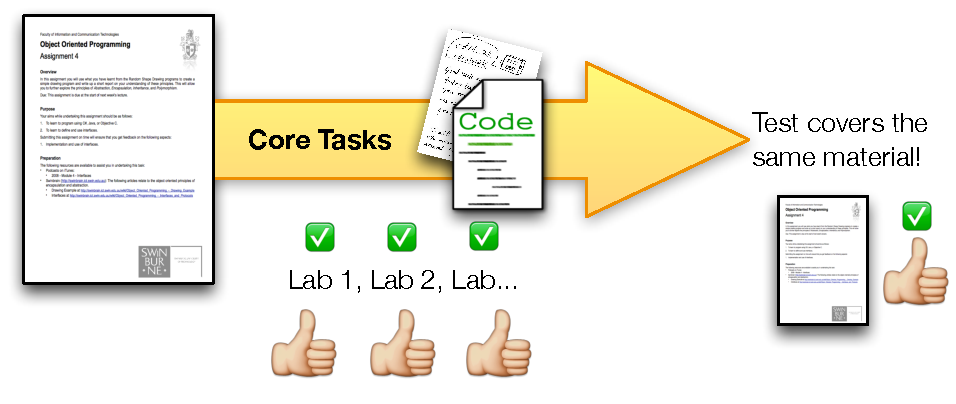
\includegraphics[width=\textwidth]{Tests}
	\caption{Tests cover aspects already presented in the tests, helping verify students completed the work themselves.}
	\label{fig:tests}
\end{figure}

As the tests only assess core competencies, the tests are marked to an exacting standard. Students can be awarded one of three grades: pass, fix or redo. 
\begin{itemize}[noitemsep,nolistsep]
	\item The \emph{pass} grade requires the large majority of the test to be correct. Small issues like minor syntax errors, or other small mistakes can be overlooked, but as a majority the work must demonstrate good mastery of the topics covered. 
	\item \emph{Fix} grades indicate some larger issues are present, but nothing critical and the work still demonstrates a sufficient mastery of the content.
	\item Where the test indicates larger issues that represent critical misunderstandings for the student, their test is marked as \emph{redo} and they must resit the test to be eligible to pass the unit. When no additional test opportunities are available this grade would indicate a \emph{Fail} result for the unit.
\end{itemize}
With both pass and fix grades, students are expected to correct all issues in their test and include the corrected versions in their portfolios. 

It is important to note that the \emph{redo} grade is awarded where critical misunderstandings are demonstrated. This is not equivalent to getting less than 50\%, or some other arbitrary percentage, of available marks. The work is assessed qualitatively, with teaching staff making expert judgements about the level of understanding being demonstrated. The response to even a single question could demonstrate critical misunderstandings, though typically this knowledge would be tested across a number of questions.

Students must include the tests in their portfolios, and the last test has to be passed in examination conditions. All tests also perform a formative role, with students needing to correct any issues themselves and resubmit the work, with the test only being signed off when students have been able to address it to the required standard.

Through a combination of weekly formative feedback, hurdle tests and interviews for higher grades, the model addresses issues of plagiarism without unduly emphasising a punitive approach. This is in keeping with \pref{itm:theory_y} from \cref{cha:guiding_principles}.

% subsection addressing_plagiarism (end)

\section{Summary} % (fold)
\label{sec:ca_summary}


%
% Overall very good - as noted, need to better link the "principles" in Ch4 to Ch3 ones?
% And perhaps rename /number these as  "guidelines"  that can refer back to in Ch 5???
%

This chapter has outlined an overall strategy for teaching introductory programming with portfolio assessment based on an objects-later approach. Using the principles from \cref{cha:guiding_principles}, a model for the development of constructively aligned units was presented. \cref{cha:example_impl} continues this work by demonstrating the application of this model in the creation and delivery of two introductory programming units.

% section summary (end)

% chapter approaching_constructive_alignment_with_portfolio_assessment (end)